% Options for packages loaded elsewhere
\PassOptionsToPackage{unicode}{hyperref}
\PassOptionsToPackage{hyphens}{url}
\PassOptionsToPackage{dvipsnames,svgnames*,x11names*}{xcolor}
%
\documentclass[
]{article}
\usepackage{amsmath,amssymb}
\usepackage{lmodern}
\usepackage{ifxetex,ifluatex}
\ifnum 0\ifxetex 1\fi\ifluatex 1\fi=0 % if pdftex
  \usepackage[T1]{fontenc}
  \usepackage[utf8]{inputenc}
  \usepackage{textcomp} % provide euro and other symbols
\else % if luatex or xetex
  \usepackage{unicode-math}
  \defaultfontfeatures{Scale=MatchLowercase}
  \defaultfontfeatures[\rmfamily]{Ligatures=TeX,Scale=1}
\fi
% Use upquote if available, for straight quotes in verbatim environments
\IfFileExists{upquote.sty}{\usepackage{upquote}}{}
\IfFileExists{microtype.sty}{% use microtype if available
  \usepackage[]{microtype}
  \UseMicrotypeSet[protrusion]{basicmath} % disable protrusion for tt fonts
}{}
\makeatletter
\@ifundefined{KOMAClassName}{% if non-KOMA class
  \IfFileExists{parskip.sty}{%
    \usepackage{parskip}
  }{% else
    \setlength{\parindent}{0pt}
    \setlength{\parskip}{6pt plus 2pt minus 1pt}}
}{% if KOMA class
  \KOMAoptions{parskip=half}}
\makeatother
\usepackage{xcolor}
\IfFileExists{xurl.sty}{\usepackage{xurl}}{} % add URL line breaks if available
\IfFileExists{bookmark.sty}{\usepackage{bookmark}}{\usepackage{hyperref}}
\hypersetup{
  pdftitle={Tarea Bloque 3},
  pdfauthor={Jose Antonio Lorencio Abril},
  colorlinks=true,
  linkcolor=red,
  filecolor=Maroon,
  citecolor=Blue,
  urlcolor=Blue,
  pdfcreator={LaTeX via pandoc}}
\urlstyle{same} % disable monospaced font for URLs
\usepackage[margin=1in]{geometry}
\usepackage{color}
\usepackage{fancyvrb}
\newcommand{\VerbBar}{|}
\newcommand{\VERB}{\Verb[commandchars=\\\{\}]}
\DefineVerbatimEnvironment{Highlighting}{Verbatim}{commandchars=\\\{\}}
% Add ',fontsize=\small' for more characters per line
\usepackage{framed}
\definecolor{shadecolor}{RGB}{248,248,248}
\newenvironment{Shaded}{\begin{snugshade}}{\end{snugshade}}
\newcommand{\AlertTok}[1]{\textcolor[rgb]{0.94,0.16,0.16}{#1}}
\newcommand{\AnnotationTok}[1]{\textcolor[rgb]{0.56,0.35,0.01}{\textbf{\textit{#1}}}}
\newcommand{\AttributeTok}[1]{\textcolor[rgb]{0.77,0.63,0.00}{#1}}
\newcommand{\BaseNTok}[1]{\textcolor[rgb]{0.00,0.00,0.81}{#1}}
\newcommand{\BuiltInTok}[1]{#1}
\newcommand{\CharTok}[1]{\textcolor[rgb]{0.31,0.60,0.02}{#1}}
\newcommand{\CommentTok}[1]{\textcolor[rgb]{0.56,0.35,0.01}{\textit{#1}}}
\newcommand{\CommentVarTok}[1]{\textcolor[rgb]{0.56,0.35,0.01}{\textbf{\textit{#1}}}}
\newcommand{\ConstantTok}[1]{\textcolor[rgb]{0.00,0.00,0.00}{#1}}
\newcommand{\ControlFlowTok}[1]{\textcolor[rgb]{0.13,0.29,0.53}{\textbf{#1}}}
\newcommand{\DataTypeTok}[1]{\textcolor[rgb]{0.13,0.29,0.53}{#1}}
\newcommand{\DecValTok}[1]{\textcolor[rgb]{0.00,0.00,0.81}{#1}}
\newcommand{\DocumentationTok}[1]{\textcolor[rgb]{0.56,0.35,0.01}{\textbf{\textit{#1}}}}
\newcommand{\ErrorTok}[1]{\textcolor[rgb]{0.64,0.00,0.00}{\textbf{#1}}}
\newcommand{\ExtensionTok}[1]{#1}
\newcommand{\FloatTok}[1]{\textcolor[rgb]{0.00,0.00,0.81}{#1}}
\newcommand{\FunctionTok}[1]{\textcolor[rgb]{0.00,0.00,0.00}{#1}}
\newcommand{\ImportTok}[1]{#1}
\newcommand{\InformationTok}[1]{\textcolor[rgb]{0.56,0.35,0.01}{\textbf{\textit{#1}}}}
\newcommand{\KeywordTok}[1]{\textcolor[rgb]{0.13,0.29,0.53}{\textbf{#1}}}
\newcommand{\NormalTok}[1]{#1}
\newcommand{\OperatorTok}[1]{\textcolor[rgb]{0.81,0.36,0.00}{\textbf{#1}}}
\newcommand{\OtherTok}[1]{\textcolor[rgb]{0.56,0.35,0.01}{#1}}
\newcommand{\PreprocessorTok}[1]{\textcolor[rgb]{0.56,0.35,0.01}{\textit{#1}}}
\newcommand{\RegionMarkerTok}[1]{#1}
\newcommand{\SpecialCharTok}[1]{\textcolor[rgb]{0.00,0.00,0.00}{#1}}
\newcommand{\SpecialStringTok}[1]{\textcolor[rgb]{0.31,0.60,0.02}{#1}}
\newcommand{\StringTok}[1]{\textcolor[rgb]{0.31,0.60,0.02}{#1}}
\newcommand{\VariableTok}[1]{\textcolor[rgb]{0.00,0.00,0.00}{#1}}
\newcommand{\VerbatimStringTok}[1]{\textcolor[rgb]{0.31,0.60,0.02}{#1}}
\newcommand{\WarningTok}[1]{\textcolor[rgb]{0.56,0.35,0.01}{\textbf{\textit{#1}}}}
\usepackage{graphicx}
\makeatletter
\def\maxwidth{\ifdim\Gin@nat@width>\linewidth\linewidth\else\Gin@nat@width\fi}
\def\maxheight{\ifdim\Gin@nat@height>\textheight\textheight\else\Gin@nat@height\fi}
\makeatother
% Scale images if necessary, so that they will not overflow the page
% margins by default, and it is still possible to overwrite the defaults
% using explicit options in \includegraphics[width, height, ...]{}
\setkeys{Gin}{width=\maxwidth,height=\maxheight,keepaspectratio}
% Set default figure placement to htbp
\makeatletter
\def\fps@figure{htbp}
\makeatother
\setlength{\emergencystretch}{3em} % prevent overfull lines
\providecommand{\tightlist}{%
  \setlength{\itemsep}{0pt}\setlength{\parskip}{0pt}}
\setcounter{secnumdepth}{-\maxdimen} % remove section numbering
\usepackage[utf8]{inputenc}
\usepackage{hyperref}
\usepackage{multirow}
\usepackage{float}
\usepackage{listings}
\usepackage{xcolor}
\ifluatex
  \usepackage{selnolig}  % disable illegal ligatures
\fi
\newlength{\cslhangindent}
\setlength{\cslhangindent}{1.5em}
\newlength{\csllabelwidth}
\setlength{\csllabelwidth}{3em}
\newenvironment{CSLReferences}[2] % #1 hanging-ident, #2 entry spacing
 {% don't indent paragraphs
  \setlength{\parindent}{0pt}
  % turn on hanging indent if param 1 is 1
  \ifodd #1 \everypar{\setlength{\hangindent}{\cslhangindent}}\ignorespaces\fi
  % set entry spacing
  \ifnum #2 > 0
  \setlength{\parskip}{#2\baselineskip}
  \fi
 }%
 {}
\usepackage{calc}
\newcommand{\CSLBlock}[1]{#1\hfill\break}
\newcommand{\CSLLeftMargin}[1]{\parbox[t]{\csllabelwidth}{#1}}
\newcommand{\CSLRightInline}[1]{\parbox[t]{\linewidth - \csllabelwidth}{#1}\break}
\newcommand{\CSLIndent}[1]{\hspace{\cslhangindent}#1}

\title{Tarea Bloque 3}
\usepackage{etoolbox}
\makeatletter
\providecommand{\subtitle}[1]{% add subtitle to \maketitle
  \apptocmd{\@title}{\par {\large #1 \par}}{}{}
}
\makeatother
\subtitle{Desarrollo de Sistemas Inteligentes}
\author{Jose Antonio Lorencio Abril}
\date{Diciembre de 2021}

\begin{document}
\maketitle

\newpage

\hypertarget{uxedndice}{%
\subsubsection{Índice}\label{uxedndice}}

\begin{itemize}
\tightlist
\item
  \protect\hyperlink{problema-1}{Problema 1}
\item
  \protect\hyperlink{problema-2}{Problema 2}
\item
  \protect\hyperlink{problema-3}{Problema 3}
\item
  \protect\hyperlink{problema-4}{Problema 4}
\item
  \protect\hyperlink{problema-5}{Problema 5}
\item
  \protect\hyperlink{bibliografuxe3uxada}{Bibliografía}
\end{itemize}

\newpage

\hypertarget{problema-1}{%
\section{Problema 1}\label{problema-1}}

\index{Problema 1} Supongamos que para una cierta aplicación definimos
unos conjuntos borrosos con estas funciones de pertenencia:
\[\mu_{A}\left(x\right)=\frac{1}{1+e^{-2\left(x-4\right)}}\]
\[\mu_{B}\left(x\right)=\frac{1}{1+e^{3\left(x-5\right)}}\] definidos
sobre el universo \(X=\left[0,10\right]\). Calcular, analítica y
gráficamente, la unión, la intersección, los complementos, las
diferencias, las dos leyes de Morgan, la ley del medio excluido y la ley
de la contradicción.

Para la resolución de este ejercicio, seguimos las definiciones
proporcionadas en los apuntes de clase
{[}\protect\hyperlink{ref-PalmaConjuntosBorrosos}{1}{]}, así como los
ejemplos resueltos
{[}\protect\hyperlink{ref-BotiaConjuntosBorrosos}{2}{]}. Primero,
notamos que los conjuntos asociados a estas relaciones de pertenencia
son:
\[A=\int_{x\in\left[0,10\right]}\mu_{A}\left(x\right)/x=\int_{x\in\left[0,10\right]}\frac{1}{1+e^{-2\left(x-4\right)}}/x\]
\[B=\int_{x\in\left[0,10\right]}\mu_{B}\left(x\right)/x=\int_{x\in\left[0,10\right]}\frac{1}{1+e^{3\left(x-5\right)}}/x\]
Que tienen la siguiente pinta:

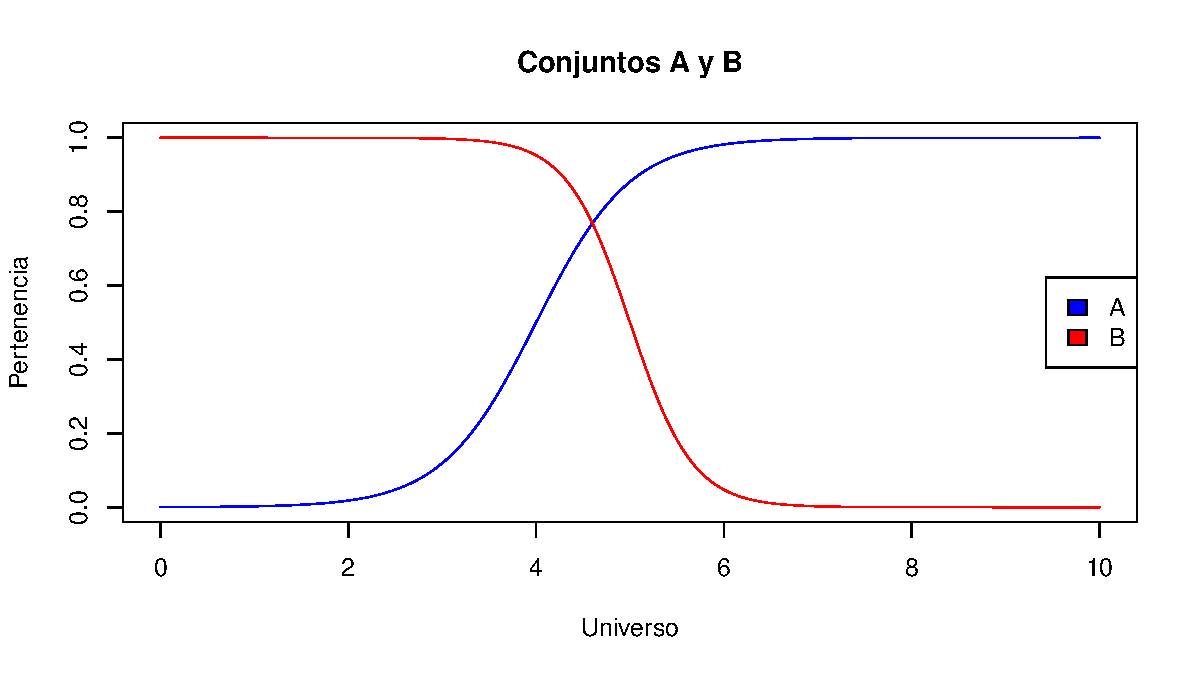
\includegraphics{tareaBloque3_files/figure-latex/unnamed-chunk-1-1.pdf}
\newpage Para calcular la \textbf{unión}, basta tomar el máximo de
ambas, gráficamente queda:

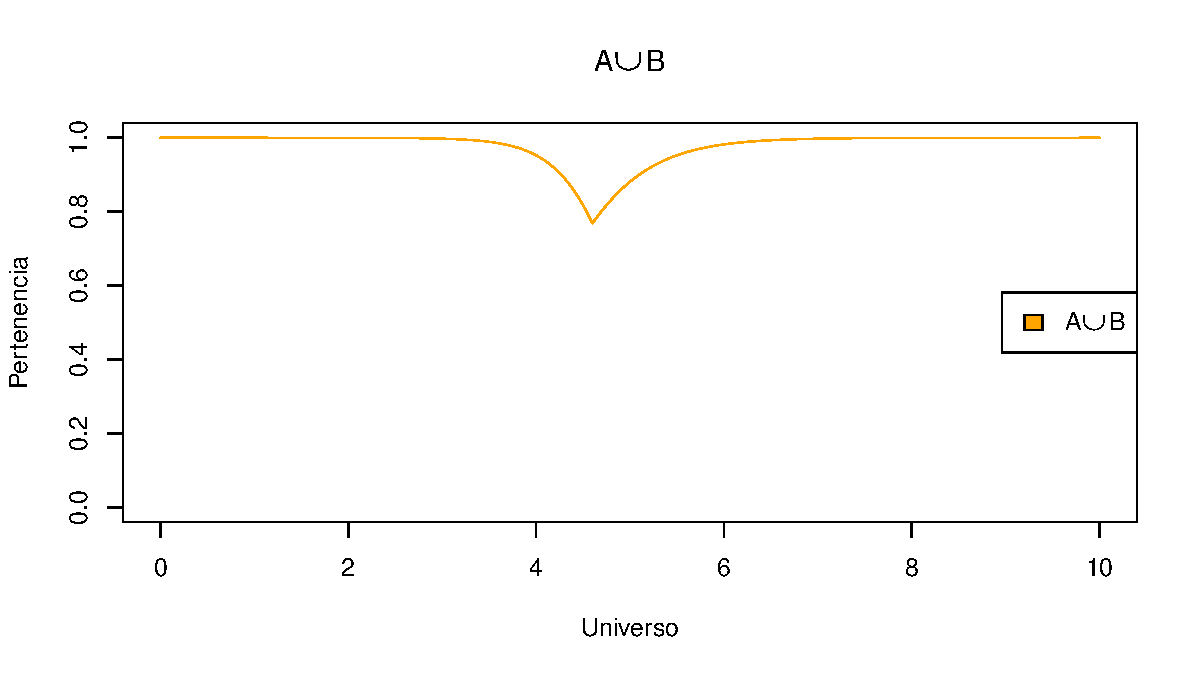
\includegraphics{tareaBloque3_files/figure-latex/unnamed-chunk-2-1.pdf}
Para hacerlo analíticamente:

\[\mu_{A}\left(x\right)\geq\mu_{B}\left(x\right)\iff\frac{1}{1+e^{-2\left(x-4\right)}}\geq\frac{1}{1+e^{3\left(x-5\right)}}\iff e^{-2\left(x-4\right)}\leq e^{3\left(x-5\right)}\iff\]
\[\iff-2\left(x-4\right)\leq3\left(x-5\right)\iff x-4\geq-\frac{3}{2}\left(x-5\right)\iff\frac{5}{2}x\geq\frac{23}{2}\iff x\geq\frac{23}{5}\]

Por tanto, es \[\mu_{A\cup B}\left(x\right)=\begin{cases}
\mu_{B}\left(x\right) & x\leq\frac{23}{5}\\
\mu_{A}\left(x\right) & x>\frac{23}{5}
\end{cases}\]

Para la \textbf{intersección}, lo que hacemos es el mínimo, que es igual
que antes, pero tomando la función recíproca:
\[\mu_{A\cap B}\left(x\right)=\begin{cases}
\mu_{A}\left(x\right) & x\leq\frac{23}{5}\\
\mu_{B}\left(x\right) & x>\frac{23}{5}
\end{cases}\]

De forma visual:

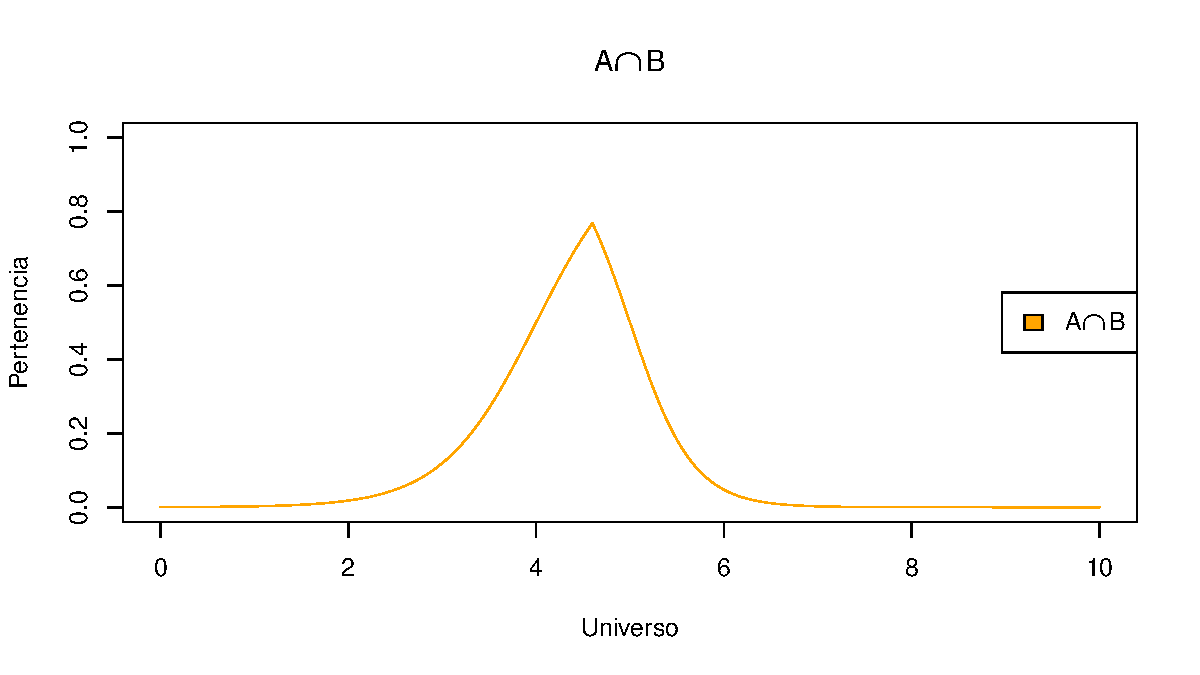
\includegraphics{tareaBloque3_files/figure-latex/unnamed-chunk-3-1.pdf}

Para el \textbf{complementario} simplement hay que tomar las funciones
de pertenencia complementarias, es decir
\[\mu_{\overline{A}}\left(x\right)=1-\mu_{A}\left(x\right)=1-\frac{1}{1+e^{-2\left(x-4\right)}}=\frac{e^{-2\left(x-4\right)}}{1+e^{-2\left(x-4\right)}}=\frac{1}{e^{2\left(x-4\right)}+1}=\frac{1}{1+e^{2\left(x-4\right)}}\]
\[\mu_{\overline{B}}\left(x\right)=1-\mu_{B}\left(x\right)=1-\frac{1}{1+e^{3\left(x-5\right)}}=\frac{e^{3\left(x-5\right)}}{1+e^{3\left(x-5\right)}}=\frac{1}{e^{-3\left(x-5\right)}+1}=\frac{1}{1+e^{-3\left(x-5\right)}}\]
y gráficamente:

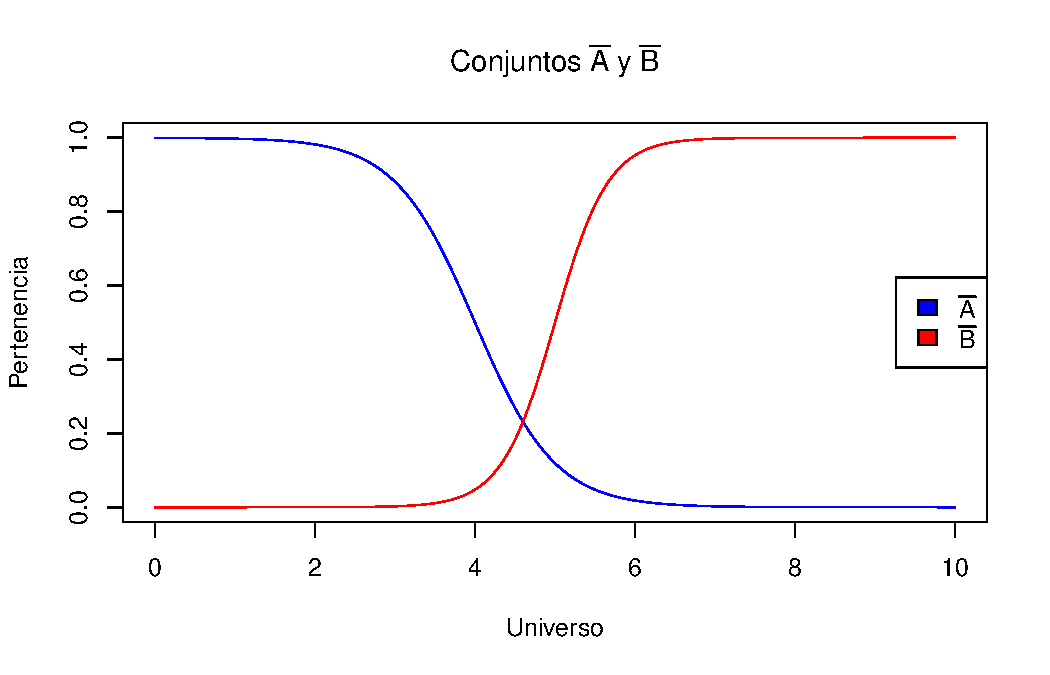
\includegraphics{tareaBloque3_files/figure-latex/unnamed-chunk-4-1.pdf}

Vamos ahora a calcular la \textbf{diferencia}:
\[\mu_{A\setminus B}\left(x\right)=\mu_{A\cap\overline{B}}\left(x\right)=\min\left\{ \mu_{A}\left(x\right),\mu_{\overline{B}}\left(x\right)\right\}\]
Primero, gráficamente:

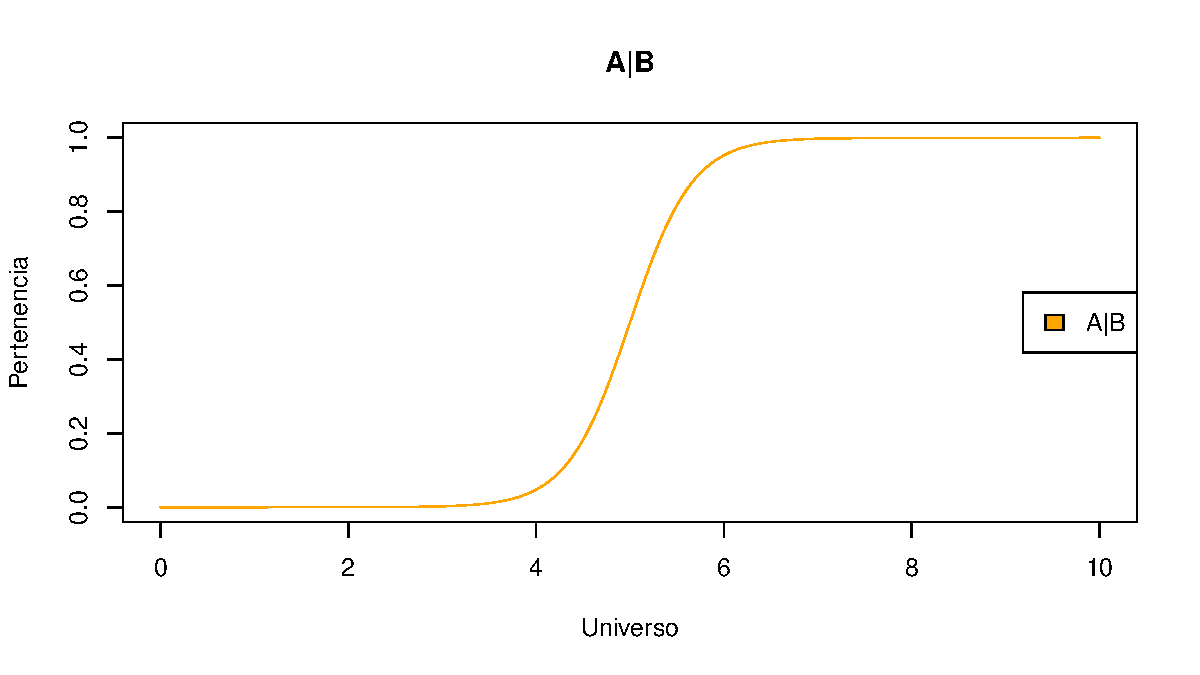
\includegraphics{tareaBloque3_files/figure-latex/unnamed-chunk-5-1.pdf}
Para hacerlo analíticamente, tenemos que calcular el máximo de las
funciones de pertenencia:
\[\mu_{A}\left(x\right)\geq\mu_{\overline{B}}\left(x\right)\iff\frac{1}{1+e^{-2\left(x-4\right)}}\geq\frac{1}{1+e^{-3\left(x-5\right)}}\iff-2\left(x-4\right)\geq-3\left(x-5\right)\iff\]
\[\iff x-4\leq\frac{3}{2}\left(x-5\right)\iff-\frac{x}{2}\leq\frac{-15+8}{2}=\frac{-7}{2}\iff-x\leq-7\iff x\geq7\]
Por lo tanto, es \[\mu_{A\setminus B}\left(x\right)=\begin{cases}
\mu_{\overline{B}}\left(x\right) & x\leq7\\
\mu_{A}\left(x\right) & x>7
\end{cases}\]

Y la otra diferencia es
\[\mu_{B\setminus A}\left(x\right)=\mu_{B\cap\overline{A}}\left(x\right)=\min\left\{ \mu_{B}\left(x\right),\mu_{\overline{A}}\left(x\right)\right\}\]

Que gráficamente queda:

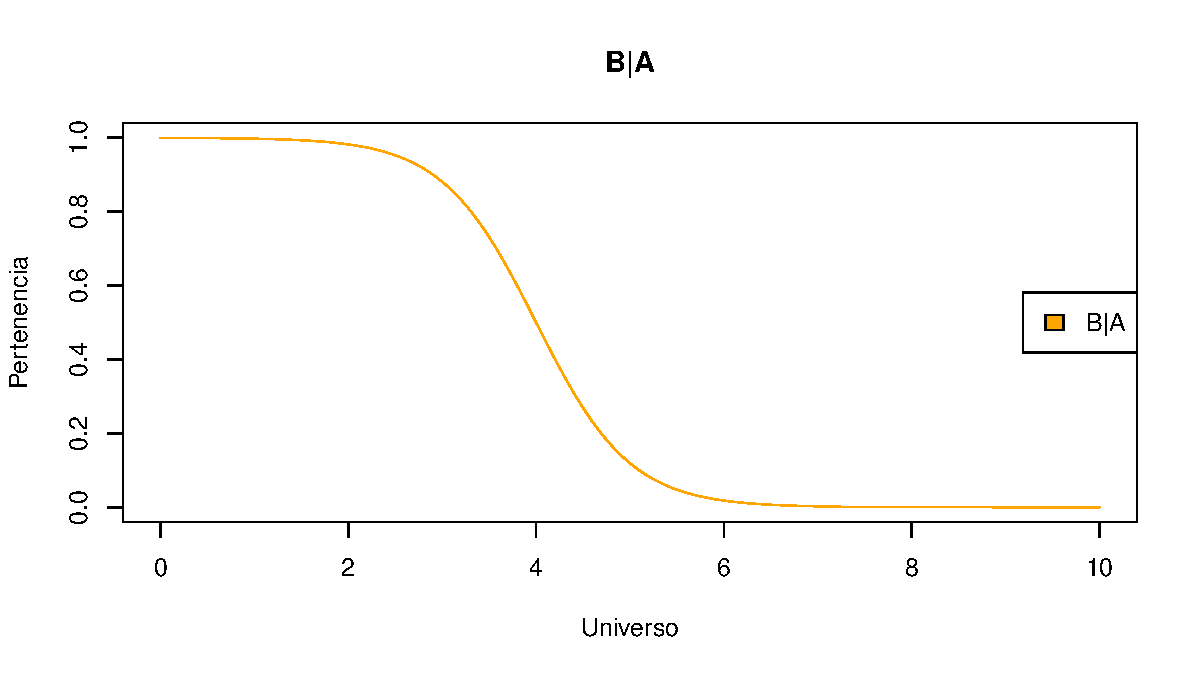
\includegraphics{tareaBloque3_files/figure-latex/unnamed-chunk-6-1.pdf}

Y analíticamente, igual que antes:
\[\mu_{B}\left(x\right)\geq\mu_{\overline{A}}\iff\frac{1}{1+e^{3\left(x-5\right)}}\geq\frac{1}{1+e^{2\left(x-4\right)}}\iff3\left(x-5\right)\leq2\left(x-4\right)\iff\]
\[\iff x-5\leq\frac{2}{3}\left(x-4\right)\iff\frac{x}{3}\leq\frac{7}{3}\iff x\leq7\]
por lo que la función de pertenencia es
\[\mu_{B\setminus A}\left(x\right)=\begin{cases}
\mu_{B}\left(x\right) & x\leq7\\
\mu_{\overline{A}}\left(x\right) & x>7
\end{cases}\]

Respecto a las \textbf{leyes de Morgan}, son
\[\mu_{\overline{A\cup B}}\left(x\right)=1-\mu_{A\cup B}\left(x\right)=\begin{cases}
1-\mu_{B}\left(x\right) & x\leq\frac{23}{5}\\
1-\mu_{A}\left(x\right) & x>\frac{23}{5}
\end{cases}=\begin{cases}
\mu_{\overline{B}}\left(x\right) & x\leq\frac{23}{5}\\
\mu_{\overline{A}}\left(x\right) & x>\frac{23}{5}
\end{cases}=\mu_{\overline{A}\cap\overline{B}}\] siendo cierta esta
igualdad, ya que se tiene la siguiente cadena de desigualdades
\[\mu_{\overline{B}}\left(x\right)\leq\mu_{\overline{A}}\left(x\right)\iff\frac{1}{1+e^{-3\left(x-5\right)}}\leq\frac{1}{1+e^{2\left(x-4\right)}}\iff-3\left(x-5\right)\geq2\left(x-4\right)\iff\]
\[\iff x-5\leq-\frac{2}{3}\left(x-4\right)\iff\frac{5}{3}x\leq\frac{23}{3}\iff x\leq\frac{23}{5}\]

Para la otra ley, repetimos un proceso análogo:
\[\mu_{\overline{A\cap B}}\left(x\right)=1-\mu_{A\cap B}\left(x\right)=\begin{cases}
\mu_{\overline{A}}\left(x\right) & x\leq\frac{23}{5}\\
\mu_{\overline{B}}\left(x\right) & x>\frac{23}{5}
\end{cases}=\mu_{\overline{A}\cup\overline{B}}\]

Y vemos ambas leyes gráficamente:

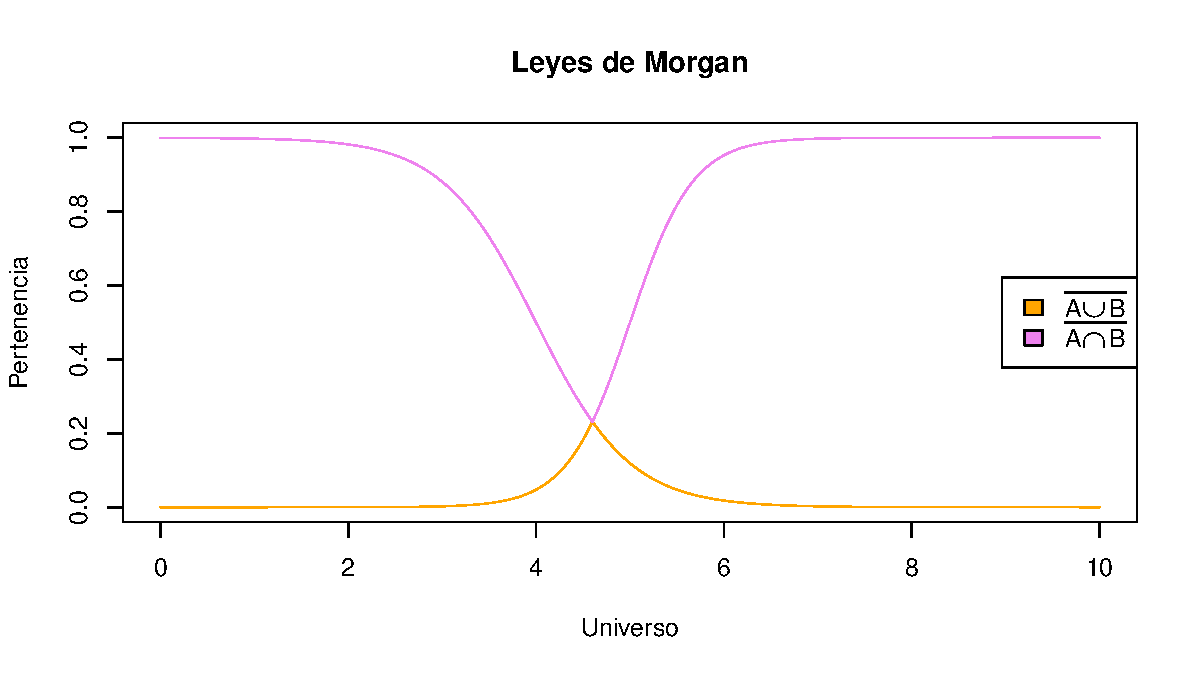
\includegraphics{tareaBloque3_files/figure-latex/unnamed-chunk-7-1.pdf}

Tratando la \textbf{ley de la contradicción}, observamos que en los
apuntes de clase {[}\protect\hyperlink{ref-PalmaConjuntosBorrosos}{1}{]}
se usa la fórmula \(A\cup\overline{A}\), pero esto no concuerda con
nuestros conocimientos de lógica. Sabemos que una contradicción se da
cuando a partir de unas premisas obtenemos una afirmación y su
contraria, y esto nos permite concluir que las premisas no son
consistentes. O sea, que para que un conjunto de premisas sea
consistente, se requiere que o bien una afirmación, o bien su contraria,
sean ciertas, pero que no lo sean ambas simultáneamente. Es decir, que
\(A\cap\overline{A}=\emptyset\). Esto podemos corroborarlo en
{[}\protect\hyperlink{ref-Stanford}{3}{]}. Así, calculamos la ley de la
contradicción para conjuntos borrosos de la siguiente forma:

\[\mu_{A\cap\overline{A}}\left(x\right)=\min\left\{ \mu_{A}\left(x\right),\mu_{\overline{A}}\left(x\right)\right\} \]
y se tiene que
\[\mu_{A}\left(x\right)\leq\mu_{\overline{A}}\left(x\right)\iff\frac{1}{1+e^{-2\left(x-4\right)}}\leq\frac{1}{1+e^{2\left(x-4\right)}}\iff-2\left(x-4\right)\geq2\left(x-4\right)\iff\]
\[4-x\geq x-4\iff8\geq2x\iff x\leq4\] por lo que la función de
pertenencia es \[\mu_{A\cap\overline{A}}\left(x\right)=\begin{cases}
\mu_{A}\left(x\right) & x\leq4\\
\mu_{\overline{A}}\left(x\right) & x>4
\end{cases}\]

Antes de hacerlo gráficamente, lo hacemos para el conjunto \(B\). Se
tiene la siguiente cadena de equivalencias:
\[\mu_{B}\left(x\right)\leq\mu_{\overline{B}}\left(x\right)\iff\frac{1}{1+e^{3\left(x-5\right)}}\leq\frac{1}{1+e^{-3\left(x-5\right)}}\iff3\left(x-5\right)\geq-3\left(x-5\right)\iff\]
\[\iff x-5\geq5-x\iff2x\geq10\iff x\geq5\] y entonces
\[\mu_{B\cap\overline{B}}\left(x\right)=\begin{cases}
\mu_{\overline{B}}\left(x\right) & x\leq5\\
\mu_{B}\left(x\right) & x>5
\end{cases}\]

Lo vemos gráficamente:

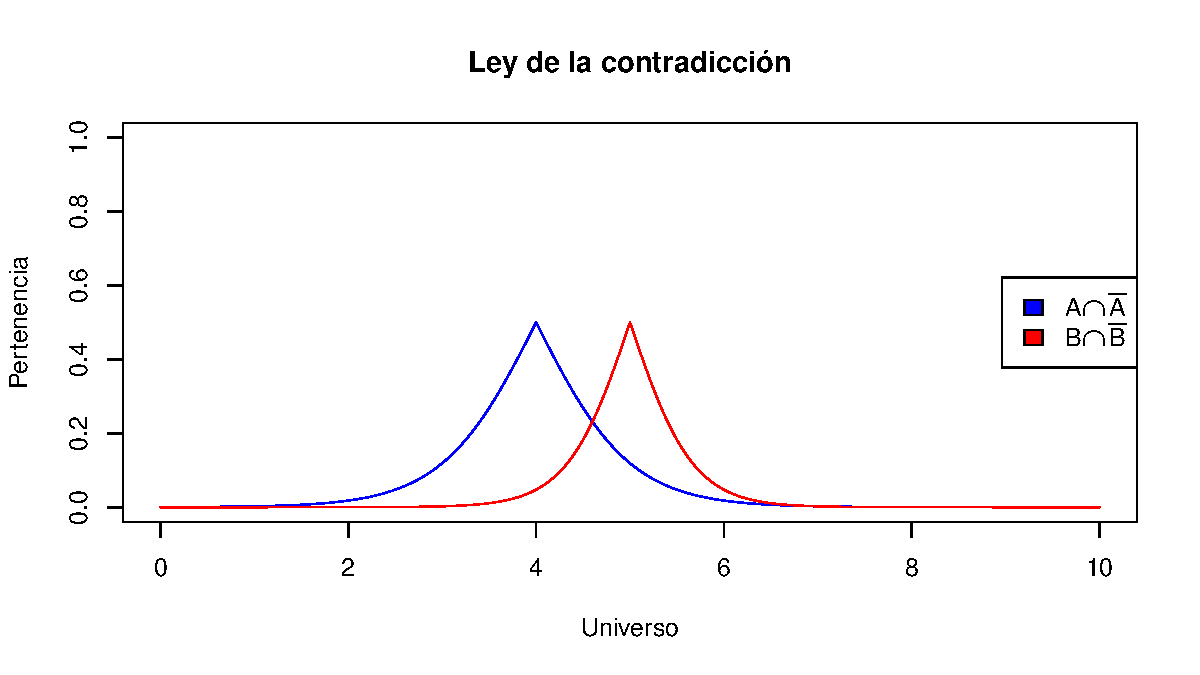
\includegraphics{tareaBloque3_files/figure-latex/unnamed-chunk-8-1.pdf}

Respecto a la \textbf{ley del medio excluido}, encontramos en los
apuntes de clase {[}\protect\hyperlink{ref-PalmaConjuntosBorrosos}{1}{]}
que debemos calcular la intersección de cada conjunto con su
complementario. De nuevo, esto no concuerda con nuestros conocimientos
previos sobre la ley del medio excluido, que asegura que bien una
proposición o bien su contraria deben ser ciertas bajo ciertas premisas,
y que estas dos opciones completan el espacio proposicional. Es decir,
que \(A\cup \overline{A}=U\). Esto lo corroboramos otra vez en
{[}\protect\hyperlink{ref-Stanford}{3}{]}, y usaremos esta fórmula para
calcularlo.

\[\mu_{A\cup\overline{A}}\left(x\right)=\mu_{\overline{\overline{A\cup\overline{A}}}}\left(x\right)=1-\mu_{\overline{A\cup\overline{A}}}\left(x\right)=1-\mu_{\overline{A}\cap A}\left(x\right)=\begin{cases}
1-\mu_{A}\left(x\right) & x\leq4\\
1-\mu_{\overline{A}}\left(x\right) & x>4
\end{cases}=\begin{cases}
\mu_{\overline{A}}\left(x\right) & x\leq4\\
\mu_{A}\left(x\right) & x>4
\end{cases}\] Obsérvese que no es más que el complementario de la ley
del medio excluido. Para \(B\), más de lo mismo:
\[\mu_{B\cup\overline{B}}\left(x\right)=\mu_{\overline{\overline{B\cup\overline{B}}}}\left(x\right)=1-\mu_{\overline{B\cup\overline{B}}}\left(x\right)=1-\mu_{\overline{B}\cap B}\left(x\right)=\begin{cases}
1-\mu_{\overline{B}}\left(x\right) & x\leq5\\
1-\mu_{B}\left(x\right) & x>5
\end{cases}=\begin{cases}
\mu_{B}\left(x\right) & x\leq5\\
\mu_{\overline{B}}\left(x\right) & x>5
\end{cases}\]

Y vemos ambos de forma gráfica:

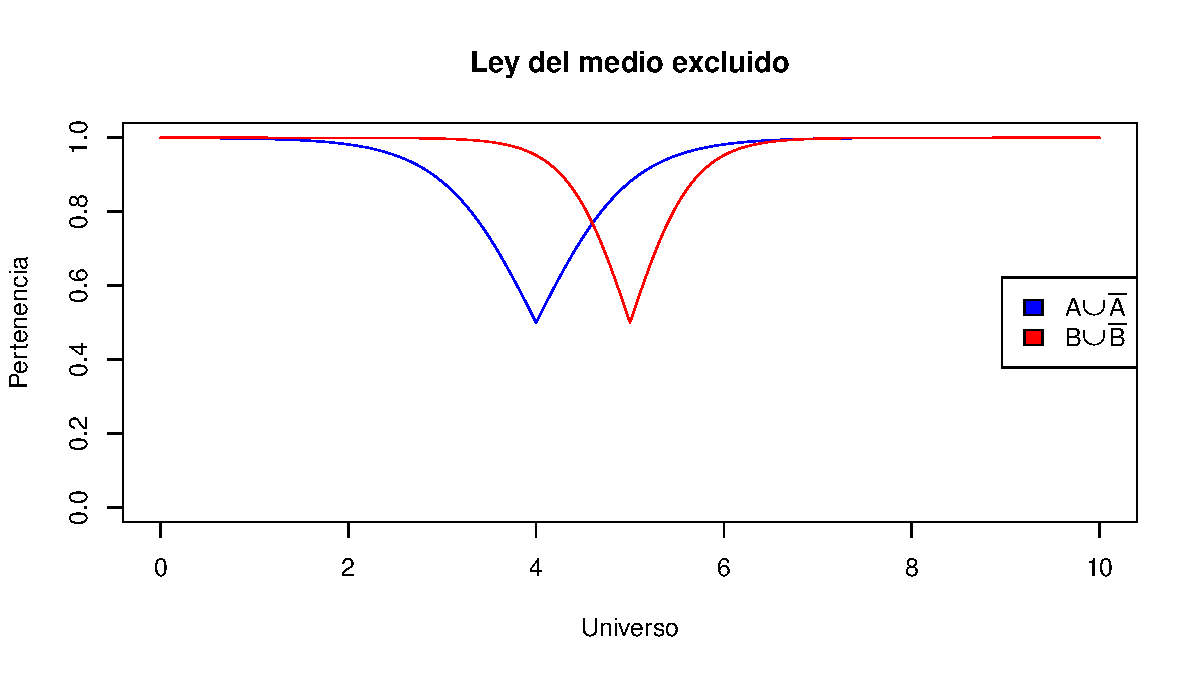
\includegraphics{tareaBloque3_files/figure-latex/unnamed-chunk-9-1.pdf}
\newpage

\hypertarget{problema-2}{%
\section{Problema 2}\label{problema-2}}

Supongamos que estamos diseñando un sistema para localizar objetos y
formas en una imagen. Un objeto determinado puede ser considerado grande
o pequeño, si el número de píxeles consecutivos en la matriz que
representa la imagen está por encima o por debajo de un determinado
valor. Si definimos el universo de discurso del número de píxeles
consecutivos por encima del valor de referencia como
\(\left[50,300\right]\), podemos definir los siguientes conjuntos
borrosos:
\["Grande"=\left\{ \frac{0}{50}+\frac{0.2}{100}+\frac{0.3}{150}+\frac{0.8}{200}+\frac{0.9}{250}+\frac{1}{300}\right\} \]
\["Pequeño"=\left\{ \frac{1}{50}+\frac{0.5}{100}+\frac{0.1}{150}+\frac{0}{200}+\frac{0}{250}+\frac{0}{300}\right\} \]
donde las distintas formas detectadas se pueden expresar en los
siguientes términos:

\begin{enumerate}
\def\labelenumi{\arabic{enumi}.}
\item
  Muy grande
\item
  Más que muy grande
\item
  No muy grande y más o menos pequeño
\item
  Muy muy grande y no pequeño
\item
  Muy pequeño y no grande
\item
  Bastante grande (=grande\(^{\frac{2}{3}}\))
\item
  Ni muy pequeño ni muy grande
\item
  Pequeño o no muy pequeño
\end{enumerate}

Calcular las funciones de pertenencia para cada uno de los términos
anteriores.

Vamos a calcular las funciones de pertenencia tal y como se definen en
los apuntes de clase
{[}\protect\hyperlink{ref-PalmaLogicaBorrosa}{4}{]}. De esta manera, y
teniendo en cuenta que \[\mu_{Grande}\left(x\right)=\begin{cases}
0 & x=50\\
0.2 & x=100\\
0.3 & x=150\\
0.8 & x=200\\
0.9 & x=250\\
1 & x=300
\end{cases}\quad \mu_{Pequeño}\left(x\right)=\begin{cases}
1 & x=50\\
0.5 & x=100\\
0.1 & x=150\\
0 & x=200\\
0 & x=250\\
0 & x=300
\end{cases}\] sería:

\begin{enumerate}
\def\labelenumi{\arabic{enumi}.}
\item
  Muy grande:
  \[\mu_{MUY\ Grande}\left(x\right)=\mu_{Grande}\left(x\right)^{2}=\begin{cases}
  0 & x=50\\
  0.04 & x=100\\
  0.09 & x=150\\
  0.64 & x=200\\
  0.81 & x=250\\
  1 & x=300
  \end{cases}\]
\item
  Más que muy grande:
  \[\mu_{MAS\ MUY\ Grande}\left(x\right)=\mu_{MUY\ Grande}\left(x\right)^{1.25}=\begin{cases}
  0 & x=50\\
  0.01788854 & x=100\\
  0.04929503 & x=150\\
  0.5724334 & x=200\\
  0.7684335 & x=250\\
  1 & x=300
  \end{cases}\]
\item
  No muy grande y más o menos pequeño: este caso tiene un poco más de
  complejidad. Primero, hacemos `no muy grande':
  \[\mu_{NO\ MUY\ Grande}\left(x\right)=1-\mu_{MUY\ Grande}\left(x\right)=\begin{cases}
  1 & x=50\\
  0.96 & x=100\\
  0.91 & x=150\\
  0.36 & x=200\\
  0.09 & x=250\\
  0 & x=300
  \end{cases}\] Ahora hacemos `más o menos pequeño':
  \[\mu_{MASMENOS\ Pequeño}\left(x\right)=\mu_{Pequeño}\left(x\right)^{\frac{1}{2}}=\begin{cases}
  1 & x=50\\
  0.7071068 & x=100\\
  0.3162278 & x=150\\
  0 & x=200\\
  0 & x=250\\
  0 & x=300
  \end{cases}\] Y lo pedido por el enunciado es su intersección, o sea,
  el mínimo de las funciones de pertenencia:
  \[\mu_{NO\ MUY\ Grande\ Y\ MASMENOS\ Pequeño}\left(x\right)=\min\left\{ \mu_{NO\ MUY\ Grande}\left(x\right),\mu_{MASMENOS\ Pequeño}\left(x\right)\right\} =\]
  \[=\begin{cases}
  1 & x=50\\
  0.7071068 & x=100\\
  0.3162278 & x=150\\
  0 & x=200\\
  0 & x=250\\
  0 & x=300
  \end{cases}=\mu_{MASMENOS\ Pequeño}\left(x\right)\] observamos que
  coincide con la función de pertenencia de `más o menos pequeño.'
\item
  Muy muy grande y no pequeño: de nuevo, calculamos cada una por
  separado y después las juntamos tomando el mínimo:
  \[\mu_{MUY\ MUY\ Grande}\left(x\right)=\mu_{MUY\ Grande}\left(x\right)^{2}=\begin{cases}
  0 & x=50\\
  0.0016 & x=100\\
  0.0081 & x=150\\
  0.4096 & x=200\\
  0.6561 & x=250\\
  1 & x=300
  \end{cases}\]
  \[\mu_{NO\ Pequeño}\left(x\right)=1-\mu_{Pequeño}\left(x\right)=\begin{cases}
  0 & x=50\\
  0.5 & x=100\\
  0.9 & x=150\\
  1 & x=200\\
  1 & x=250\\
  1 & x=300
  \end{cases}\] y tomando el mínimo es:
  \[\mu_{MUY\ MUY\ Grande\ Y\ NO\ Pequeño}\left(x\right)=\begin{cases}
  0 & x=50\\
  0.0003199999 & x=100\\
  0.00243 & x=150\\
  0.32768 & x=200\\
  0.59049 & x=250\\
  1 & x=300
  \end{cases}=\mu_{MUY\ MUY\ Grande}\left(x\right)\] Que coincide con
  ser `muy muy grande.'
\item
  Muy pequeño y no grande:
  \[\mu_{MUY\ Pequeño}\left(x\right)=\begin{cases}
  1 & x=50\\
  0.25 & x=100\\
  0.01 & x=150\\
  0 & x=200\\
  0 & x=250\\
  0 & x=300
  \end{cases} \qquad \mu_{NO\ Grande}\left(x\right)=\begin{cases}
  1 & x=50\\
  0.8 & x=100\\
  0.7 & x=150\\
  0.2 & x=200\\
  0.1 & x=250\\
  0 & x=300
  \end{cases}\]
\end{enumerate}

Y entonces
\[\mu_{MUY\ Pequeño\ Y\ NO\ Grande}\left(x\right)=\begin{cases}
1 & x=50\\
0.25 & x=100\\
0.01 & x=150\\
0 & x=200\\
0 & x=250\\
0 & x=300
\end{cases}=\mu_{MUY\ Pequeño}\left(x\right)\]

\begin{enumerate}
\def\labelenumi{\arabic{enumi}.}
\setcounter{enumi}{5}
\item
  Bastante grande: tal y como indica el enunciado, es
  \[\mu_{BASTANTE\ Grande}\left(x\right)=\mu_{Grande}\left(x\right)^{\frac{2}{3}}=\begin{cases}
  0 & x=50\\
  0.3419952 & x=100\\
  0.4481405 & x=150\\
  0.8617739 & x=200\\
  0.9321698 & x=250\\
  1 & x=300
  \end{cases}\]
\item
  Ni muy pequeño ni muy grande: esto es lo mismo que decir `no muy
  pequeño y no muy grande,' por lo que calculamos:
  \[\mu_{NO\ MUY\ Pequeño}\left(x\right)=\begin{cases}
  0 & x=50\\
  0.75 & x=100\\
  0.99 & x=150\\
  1 & x=200\\
  1 & x=250\\
  1 & x=300
  \end{cases} \quad \mu_{NO\ MUY\ Grande}\left(x\right)=\begin{cases}
  1 & x=50\\
  0.96 & x=100\\
  0.91 & x=150\\
  0.36 & x=200\\
  0.19 & x=250\\
  0 & x=300
  \end{cases}\] y su intersección queda:
  \[\mu_{NO\ MUY\ Pequeño\ Y\ NO\ MUY\ Grande}\left(x\right)=\begin{cases}
  0 & x=50\\
  0.75 & x=100\\
  0.91 & x=150\\
  0.36 & x=200\\
  0.19 & x=250\\
  0 & x=300
  \end{cases}\]
\item
  Pequeño o no muy pequeño: en este caso debemos tomar el máximo, y las
  dos funciones de pertenencia involucradas ya las conocemos:
  \[\mu_{Pequeño\ O\ NO\ MUY\ Pequeño}\left(x\right)=\max\left\{ \mu_{Pequeño}\left(x\right),\mu_{NO\ MUY\ Pequeño}\left(x\right)\right\} =\begin{cases}
  1 & x=50\\
  0.75 & x=100\\
  0.99 & x=150\\
  1 & x=200\\
  1 & x=250\\
  1 & x=300
  \end{cases}\]
\end{enumerate}

\newpage

\hypertarget{problema-3}{%
\section{Problema 3}\label{problema-3}}

Queremos desarrollar un sistema controlador para regular la temperatura
de una habitación. Una vez analizado el problema, hemos llegado a la
conclusión de que solo con una regla podemos alcanzar el objetivo:
``Cuando la habitación está caliente, endría la habitación activando el
ventilador a una velocidad alta.'' Es decir, podemos codiifcar el
funcionamiento del controlador con la regla:

\[\boldsymbol{SI}\ la\ temperatura\ es\ ALTA\ \boldsymbol{ENTONCES}\ la\ velocidad\ de\ giro\ tiene\ que\ ser\ \boldsymbol{RÁPIDA}\]

Para utilizar esta regla se definen los conjuntos borrosos ``Temperatura
alta,'' \(C\), sobre el universo formado por las temperaturas en ºC, y
el conjunto ``rápida,'' sobre el universo de velocidades de giro en 1000
rpm:

\[C="Temperatura\ alta"=\left\{ \frac{0.0}{16}+\frac{0.1}{20}+\frac{0.7}{25}+\frac{0.9}{30}+\frac{1.0}{35}\right\} \]
\[R="rápida"=\left\{ \frac{0.0}{0}+\frac{0.2}{1}+\frac{0.5}{2}+\frac{0.9}{3}+\frac{1.0}{4}\right\} \]

\begin{enumerate}
\def\labelenumi{\arabic{enumi}.}
\item
  Para los anteriores conjuntos borrosos construir la relación de
  implicación utilizando:

  \begin{itemize}
  \item
    La interpretación clásica de la implicación
  \item
    La implicación de Mandami
  \item
    La implicación de Larsen
  \item
    Comparar los anteriores resultados
  \end{itemize}
\item
  Supongamos que modificamos el antecedente de la regla introduciendo el
  siguiente conjunto borroso:
  \[C'="Moderadamente\ alta"=\left\{ \frac{0.0}{16}+\frac{0.2}{20}+\frac{1.0}{25}+\frac{1.0}{30}+\frac{1.0}{35}\right\} \]
  calcular el conjunto borroso que describe la velocidad del ventilador
  utilizando:

  \begin{itemize}
  \item
    La composición max-min para las implicaciones clásica y Mandami
  \item
    La composición max-producto para la implicación Larsen
  \item
    En el caso de las implicaciones de Mandami y Larsen utiliza la
    expresión basada en el grado de satisfacción
  \end{itemize}
\item
  Supongamos que modificamos el consecuente de la regla introduciendo el
  siguiente conjunto borroso:
  \[R'="Moderamente\ rápida"=\left\{ \frac{0.0}{0}+\frac{0.4}{1}+\frac{0.7}{2}+\frac{1.0}{3}+\frac{1.0}{4}\right\} \]
  calcular el conjunto borroso que describe la temperatura de la
  habitación utilizando:

  \begin{itemize}
  \item
    La composición max-min para las implicaciones clásica y Mandami
  \item
    La composición max-producto para la implicación Larsen
  \end{itemize}
\end{enumerate}

Empecemos por el principio:

\begin{enumerate}
\def\labelenumi{\arabic{enumi}.}
\item
  Tal y como se explica en
  {[}\protect\hyperlink{ref-BotiaPalmaImplicaciones}{5}{]} o en
  {[}\protect\hyperlink{ref-PalmaLogicaBorrosa}{4}{]}, la implicación
  clásica es la de Dienes-Rescher, y consiste en interpretar
  \(p\rightarrow q\) como \(\neg p\lor q\). Por lo tanto,
  \[I_{Clasica}\left(c,r\right)=\mu_{C\rightarrow R}\left(c,r\right)=\max\left\{ 1-\mu_{C}\left(c\right),\mu_{R}\left(r\right)\right\} \]
  y entonces, la relación borrosa resultante es:
  \[\widetilde{R_{Clasica}}=\begin{array}{cccccc}
   & 0 & 1 & 2 & 3 & 4\\
  16 & 1 & 1 & 1 & 1 & 1\\
  20 & 0.9 & 0.9 & 0.9 & 0.9 & 1\\
  25 & 0.3 & 0.3 & 0.5 & 0.9 & 1\\
  30 & 0.1 & 0.2 & 0.5 & 0.9 & 1\\
  35 & 0 & 0.2 & 0.5 & 0.9 & 1
  \end{array}\] La implicación de Mandani es la que responde a la
  fórmula:
  \[I_{M}\left(c,r\right)=\mu_{C\rightarrow R}\left(c,r\right)=\min\left\{ \mu_{C}\left(c\right),\mu_{R}\left(r\right)\right\} \]
  por lo que obtenemos la relación borrosa:
  \[\widetilde{R_{M}}=\begin{array}{cccccc}
   & 0 & 1 & 2 & 3 & 4\\
  16 & 0 & 0 & 0 & 0 & 0\\
  20 & 0 & 0.1 & 0.1 & 0.1 & 0.1\\
  25 & 0 & 0.2 & 0.5 & 0.7 & 0.7\\
  30 & 0 & 0.2 & 0.5 & 0.9 & 0.9\\
  35 & 0 & 0.2 & 0.5 & 0.9 & 1
  \end{array}\] Respecto a la implicación de Larsen, es la
  correspondiente a la t-norma del producto:
  \[I_{L}\left(c,r\right)=\mu_{C\rightarrow R}\left(c,r\right)=\mu_{C}\left(r\right)\cdot\mu_{R}\left(r\right)\]
  que nos da la siguiente relación:
  \[\widetilde{R_{L}}=\begin{array}{cccccc}
   & 0 & 1 & 2 & 3 & 4\\
  16 & 0 & 0 & 0 & 0 & 0\\
  20 & 0 & 0.02 & 0.05 & 0.09 & 0.1\\
  25 & 0 & 0.14 & 0.35 & 0.63 & 0.7\\
  30 & 0 & 0.18 & 0.45 & 0.81 & 0.9\\
  35 & 0 & 0.2 & 0.5 & 0.9 & 1
  \end{array}\] Como puede observarse, se verifica que
  \(\widetilde{R_{L}}\left(c,r\right)\leq\widetilde{R_{M}}\left(c,r\right)\leq\widetilde{R_{Clasica}}\left(c,r\right),\forall c\in C,\forall r\in R\).
  Esto sucede siempre entre estos tres modelos de implicaciones, por la
  desigualdad general
  \[a\cdot b\leq\min\left\{ a,b\right\} \leq\max\left\{ a,b\right\} ,\ \forall a,b\in\left[0,1\right]\]
  y se traduce en que, a la hora de hacer inferencia, la implicación de
  Larsen proporcionará un conjunto borroso con una función de
  pertenencia menor o igual que la obtenida al usar Mandani, y esta, a
  su vez, será menor que la obtenida con la implicación clásica.
\item
  Como se explica en {[}\protect\hyperlink{ref-PalmaInferencia}{6}{]} y
  se ejemplifica en
  {[}\protect\hyperlink{ref-BotiaPalmaImplicaciones}{5}{]}, la
  composición \textbf{max-min} será: \(C'\circ R\), donde \(R\) será la
  relación a aplicar, y la composición será:
  \[\mu_{R'}\left(r\right)=\max_{\left(c,r\right)\in C\times R}\left\{ \min\left\{ \mu_{C'}\left(c\right),\widetilde{R}\left(c,r\right)\right\} \right\} \]
  En el caso de la implicación clásica, quedará:
  \[R_C'=C'\circ\widetilde{R_{C}}=\left[\frac{0}{16}+\frac{0.2}{20}+\frac{1}{25}+\frac{1}{30}+\frac{1}{35}\right]\times\begin{array}{cccccc}
   & 0 & 1 & 2 & 3 & 4\\
  16 & 1 & 1 & 1 & 1 & 1\\
  20 & 0.9 & 0.9 & 0.9 & 0.9 & 1\\
  25 & 0.3 & 0.3 & 0.5 & 0.9 & 1\\
  30 & 0.1 & 0.2 & 0.5 & 0.9 & 1\\
  35 & 0 & 0.2 & 0.5 & 0.9 & 1
  \end{array}=\]
  \[=\left[\frac{\max\left\{ 0,0.2,0.3,0.1\right\} }{0}+\frac{\max\left\{ 0.0,2,0.3\right\} }{1}+\frac{\max\left\{ 0,0.2,0.5\right\} }{2}+\frac{\max\left\{ 0,0.2,0.9\right\} }{3}+\frac{\max\left\{ 0,0.2,1\right\} }{4}\right]=\]
  \[=\left[\frac{0.3}{0}+\frac{0.3}{1}+\frac{0.5}{2}+\frac{0.9}{3}+\frac{1}{4}\right]
  \]
\end{enumerate}

En el caso de la implicación de Mandani, tenemos
\[R_{M}'=C'\circ\widetilde{R_{M}}=\left[\frac{0}{16}+\frac{0.2}{20}+\frac{1}{25}+\frac{1}{30}+\frac{1}{35}\right]\times\begin{array}{cccccc}
 & 0 & 1 & 2 & 3 & 4\\
16 & 0 & 0 & 0 & 0 & 0\\
20 & 0 & 0.1 & 0.1 & 0.1 & 0.1\\
25 & 0 & 0.2 & 0.5 & 0.7 & 0.7\\
30 & 0 & 0.2 & 0.5 & 0.9 & 0.9\\
35 & 0 & 0.2 & 0.5 & 0.9 & 1
\end{array}=\]
\[=\left[\frac{\max\left\{ 0\right\} }{0}+\frac{\max\left\{ 0,0.1,0.2\right\} }{1}+\frac{\max\left\{ 0,0.1,0.5\right\} }{2}+\frac{\max\left\{ 0,0.1,0.7,0.9\right\} }{3}+\frac{\max\left\{ 0,0.1,0.7,0.9,1\right\} }{4}\right]=\]
\[\left[\frac{0}{0}+\frac{0.2}{1}+\frac{0.5}{2}+\frac{0.9}{3}+\frac{1}{4}\right]\]

Respecto a la composición max-producto para la implicación de Larsen,
debemos hacer la operación
\[\mu_{R'}\left(r\right)=\max_{\left(c,r\right)\in C\times R}\left\{ \mu_{C'}\left(c\right)\cdot\widetilde{R_{L}}\left(c,r\right)\right\} \]
y obtenemos el conjunto borroso
\[R_{L}'=C'\circ\widetilde{R_{L}}=\left[\frac{0}{16}+\frac{0.2}{20}+\frac{1}{25}+\frac{1}{30}+\frac{1}{35}\right]\times\begin{array}{cccccc}
 & 0 & 1 & 2 & 3 & 4\\
16 & 0 & 0 & 0 & 0 & 0\\
20 & 0 & 0.02 & 0.05 & 0.09 & 0.1\\
25 & 0 & 0.14 & 0.35 & 0.63 & 0.7\\
30 & 0 & 0.18 & 0.45 & 0.81 & 0.9\\
35 & 0 & 0.2 & 0.5 & 0.9 & 1
\end{array}=\]
\[=\left[\frac{\max\left\{ 0\right\} }{0}+\frac{\max\left\{ 0,0.04,0.14,0.18,0.2\right\} }{1}+\frac{\max\left\{ 0,0.01,0.35,0.45,0.5\right\} }{2}+...\right]=\]
\[=\left[...+\frac{\max\left\{ 0.,0.018,0.63,0.81,0.9\right\} }{3}+\frac{\max\left\{ 0,0.02,0.7,0.9,1\right\} }{4}\right]=\]
\[=\left[\frac{0}{0}+\frac{0.2}{1}+\frac{0.5}{2}+\frac{0.9}{3}+\frac{1}{4}\right]\]

Por último, repetimos las implicaciones de Mandami y Larsen utilizando
el grado de satisfacción, que se define como
\[DOF\left(C',C\right)=\max_{c\in C}\left\{ \mu_{C'}\left(c\right)*\mu_{C}\left(c\right)\right\} \]
con
\[\mu_{R'}\left(r\right)=\min_{\left(c,r\right)\in C\times R}\left\{ DOF\left(C',C\right),\mu_{R}\left(r\right)\right\} \]
De este modo, sería
\[DOF_{M}\left(C',C\right)=\max_{c\in C}\left\{ \min\left\{ \mu_{C'}\left(c\right),\mu_{C}\left(c\right)\right\} \right\} =\max\left\{ 0,0.1,0.7,0.9,1\right\} =1\]
Y entonces resulta
\[R_M'=\left[\frac{\min\left\{ 1,\mu_{R}\left(0\right)\right\} }{0}+\frac{\min\left\{ 1,\mu_{R}\left(1\right)\right\} }{1}+\frac{\min\left\{ 1,\mu_{R}\left(2\right)\right\} }{2}+\frac{\min\left\{ 1,\mu_{R}\left(3\right)\right\} }{3}+\frac{\min\left\{ 1,\mu_{R}\left(4\right)\right\} }{4}\right]=\]
\[=\left[\frac{0}{0}+\frac{0.2}{1}+\frac{0.5}{2}+\frac{0.9}{3}+\frac{1}{4}\right]\]
que, como era de esperar, coincide con el resultado obtenido
anteriormente. Para Larsen, el DOF es:
\[DOF_{L}\left(C',C\right)=\max_{c\in C}\left\{ \mu_{C'}\left(c\right)\cdot\mu_{C}\left(c\right)\right\} =\max_{c\in C}\left\{ 0,0.02,0.7,0.9,1\right\} =1\]
Por lo que obtenemos el mismo resultado y, por tanto, el mismo conjunto
\(R'\), tal y como esperábamos.

\begin{enumerate}
\def\labelenumi{\arabic{enumi}.}
\setcounter{enumi}{2}
\tightlist
\item
  Para este último apartado del problema, tenemos que hacer lo mismo que
  en el anterior, pero la composición se hace por el otro lado. Es
  decir: \[C'=\widetilde{R}\circ R'^{T}\] donde la \(T\) indica la
  traspuesta, y la composición será la pertinente en cada caso.
\end{enumerate}

Para la implicación clásica:
\[C_{C}'=\widetilde{R_{C}}\circ R'^{T}=\begin{array}{cccccc}
 & 0 & 1 & 2 & 3 & 4\\
16 & 1 & 1 & 1 & 1 & 1\\
20 & 0.9 & 0.9 & 0.9 & 0.9 & 1\\
25 & 0.3 & 0.3 & 0.5 & 0.9 & 1\\
30 & 0.1 & 0.2 & 0.5 & 0.9 & 1\\
35 & 0 & 0.2 & 0.5 & 0.9 & 1
\end{array}\times\left[\begin{array}{c}
\frac{0}{0}\\
\frac{0.4}{1}\\
\frac{0.7}{2}\\
\frac{1}{3}\\
\frac{1}{4}
\end{array}\right]=\]
\[=\left[\frac{\max\left\{ 0,0.4,0.7,1,1\right\} }{16}+\frac{\max\left\{ 0,0.4,0.7,0.9,1\right\} }{20}+\frac{\max\left\{ 0,0.3,0.5,0.9,1\right\} }{25}+...\right]=\]
\[=\left[...+\frac{\max\left\{ 0,0.2,0.5,0.9,1\right\} }{30}+\frac{\max\left\{ 0,0.2,0.5,0.9,1\right\} }{35}\right]=\]
\[=\left[\frac{1}{16}+\frac{1}{20}+\frac{1}{25}+\frac{1}{30}+\frac{1}{35}\right]\]

En cuanto a la implicación de Mandami:
\[C_{M}'=\widetilde{R_{M}}\circ R'^{T}=\begin{array}{cccccc}
 & 0 & 1 & 2 & 3 & 4\\
16 & 0 & 0 & 0 & 0 & 0\\
20 & 0 & 0.1 & 0.1 & 0.1 & 0.1\\
25 & 0 & 0.2 & 0.5 & 0.7 & 0.7\\
30 & 0 & 0.2 & 0.5 & 0.9 & 0.9\\
35 & 0 & 0.2 & 0.5 & 0.9 & 1
\end{array}\times\left[\begin{array}{c}
\frac{0}{0}\\
\frac{0.4}{1}\\
\frac{0.7}{2}\\
\frac{1}{3}\\
\frac{1}{4}
\end{array}\right]=\left[\frac{0}{16}+\frac{0.1}{20}+\frac{0.7}{25}+\frac{0.9}{30}+\frac{1}{35}\right]\]

Por último, hacemos la de Larsen:
\[C_{L}'=\widetilde{R_{L}}\circ R'^{T}=\begin{array}{cccccc}
 & 0 & 1 & 2 & 3 & 4\\
16 & 0 & 0 & 0 & 0 & 0\\
20 & 0 & 0.02 & 0.05 & 0.09 & 0.1\\
25 & 0 & 0.14 & 0.35 & 0.63 & 0.7\\
30 & 0 & 0.18 & 0.45 & 0.81 & 0.9\\
35 & 0 & 0.2 & 0.5 & 0.9 & 1
\end{array}\times\left[\begin{array}{c}
\frac{0}{0}\\
\frac{0.4}{1}\\
\frac{0.7}{2}\\
\frac{1}{3}\\
\frac{1}{4}
\end{array}\right]=\left[\frac{0}{16}+\frac{0.1}{20}+\frac{0.7}{25}+\frac{0.9}{30}+\frac{1}{35}\right]\]

\newpage

\hypertarget{problema-4}{%
\section{Problema 4}\label{problema-4}}

Se nos ha pedido diseñar un sistema de inferencia borroso para simular
el descenso final y las maniobras de aterrizaje de un avión. La
velocidad de descenso es proporcional al cuadrado de la altitud. De esta
forma, para altitudes grandes se requiere una velocidad de descenso
grande. A medida que la altitud disminuye, la velocidad de descenso va
disminuyendo. En el límite, la altitud se hará infinitamente pequeña y
la velocidad tenderá a cero De esta forma el avión descenderá
bruscamente pero aterrizará suavemente para evitar daños.

Las dos variables de estado para esta simulación son la altitud, h, y la
velocidad de descenso, v. La variable de control obtenida como salida
del SIB será la fuerza que, una vez aplicada al avión, modificará su
altitud h, y su velocidad v. Para el diseño del controlador borroso se
han definido las siguientes variables lingüísticas:

\begin{itemize}
\tightlist
\item
  \textbf{Altitud}, definida sobre el universo de discurso
  \(X_{1}=\left[0,1000\right]\) (en pies), a través de los siguientes
  conjuntos borrosos:
\end{itemize}

\[Grande\left(L\right)=\mu_{L}\left(x\right)=\left\{ \frac{0}{500}+\frac{0.2}{600}+\frac{0.4}{700}+\frac{0.6}{800}+\frac{0.8}{900}+\frac{1}{1000}\right\} \]
\[Media\left(M\right)=\mu_{M}\left(x\right)=\left\{ \frac{0}{300}+\frac{0.2}{400}+\frac{0.4}{500}+\frac{0.6}{600}+\frac{0.8}{700}+\frac{1}{800}+\frac{0.8}{900}+\frac{0.6}{1000}\right\} \]
\[Pequeña\left(S\right)=\mu_{S}\left(x\right)=\left\{ \frac{0.4}{0}+\frac{0.6}{100}+\frac{0.8}{200}+\frac{1}{300}+\frac{0.8}{400}+\frac{0.6}{500}+\frac{0.4}{600}+\frac{0.2}{700}+\frac{0}{800}\right\} \]
\[Cerca\_cero\left(NZ\right)=\mu_{NZ}\left(x\right)=\left\{ \frac{1}{0}+\frac{0.8}{100}+\frac{0.6}{200}+\frac{0.4}{300}+\frac{0.2}{400}+\frac{0}{500}\right\} \]

\begin{itemize}
\tightlist
\item
  \textbf{Velocidad}, definida sobre el universo
  \(X_{2}=\left[-30,30\right]\) (pies/seg) a través de los siguientes
  conjuntos borrosos:
\end{itemize}

\[alta\ ascendente\left(UL\right)=\mu_{UL}\left(x\right)=\left\{ \frac{0}{10}+\frac{0.5}{15}+\frac{1}{20}+\frac{1}{25}+\frac{1}{30}\right\} \]
\[baja\ ascendente\left(US\right)=\mu_{US}\left(x\right)=\left\{ \frac{0}{0}+\frac{0.5}{5}+\frac{1}{10}+\frac{0.5}{15}+\frac{0}{20}\right\} \]
\[cero\left(Z\right)=\mu_{Z}\left(x\right)=\left\{ \frac{0}{-10}+\frac{0.5}{-5}+\frac{1}{0}+\frac{0.5}{5}+\frac{0}{10}\right\} \]
\[baja\ descendente\left(DS\right)=\mu_{DS}\left(x\right)=\left\{ \frac{0}{-20}+\frac{0.5}{-15}+\frac{1}{-10}+\frac{0.5}{-5}+\frac{0}{0}\right\} \]
\[alta\ descendente\left(DL\right)=\mu_{DL}\left(x\right)=\left\{ \frac{1}{-30}+\frac{1}{-25}+\frac{1}{-20}+\frac{0.5}{-15}+\frac{0}{-10}\right\} \]

\begin{itemize}
\tightlist
\item
  \textbf{Fuerza de control}, definida sobre el universo
  \(X_{3}=\left[-30,30\right]\) (libras), a través de los siguientes
  conjuntos borrosos:
\end{itemize}

\[alta\ ascendente\left(UL\right)=\mu_{UL}\left(x\right)=\left\{ \frac{0}{10}+\frac{0.5}{15}+\frac{1}{20}+\frac{1}{25}+\frac{1}{30}\right\} \]
\[baja\ ascendente\left(US\right)=\mu_{US}\left(x\right)=\left\{ \frac{0}{0}+\frac{0.5}{5}+\frac{1}{10}+\frac{0.5}{15}+\frac{0}{20}\right\} \]
\[cero\left(Z\right)=\mu_{Z}\left(x\right)=\left\{ \frac{0}{-10}+\frac{0.5}{-5}+\frac{1}{0}+\frac{0.5}{5}+\frac{0}{10}\right\} \]
\[baja\ descendente\left(DS\right)=\mu_{DS}\left(x\right)=\left\{ \frac{0}{-20}+\frac{0.5}{-15}+\frac{1}{-10}+\frac{0.5}{-5}+\frac{0}{0}\right\} \]
\[alta\ descendente\left(DL\right)=\mu_{DL}\left(x\right)=\left\{ \frac{1}{-30}+\frac{1}{-25}+\frac{1}{-20}+\frac{0.5}{-15}+\frac{0}{-10}\right\} \]

y el siguiente conjunto de reglas:

\begin{itemize}
\item
  \textbf{REGLA-1}: \textbf{Si} la altitud es \textbf{muy grande y} la
  velocidad es \textbf{muy alta ascendente entonces} la fuerza debe ser
  \textbf{alta descendente}
\item
  \textbf{REGLA-2}: \textbf{Si} la altitud es \textbf{media y} la
  velocidad es \textbf{baja ascendente entonces} la fuerza debe ser
  \textbf{baja descendente}
\item
  \textbf{REGLA-3}: \textbf{Si} la altitud es \textbf{algo media y} la
  velocidad es \textbf{algo alta ascendente entonces} la fuerza debe ser
  \textbf{baja descendente}
\item
  \textbf{REGLA-4}: \textbf{Si} la altitud es \textbf{pequeña y} la
  velocidad es \textbf{baja descendente entonces} la fuerza debe ser
  \textbf{baja ascendente}
\item
  \textbf{REGLA-5}: \textbf{Si} la altitud es \textbf{cercana a cero o}
  la velocidad es \textbf{cero entonces} la fuerza debe ser
  \textbf{cero}
\item
  \textbf{REGLA-6}: \textbf{Si} la altitud \textbf{no} es
  \textbf{cercana a cero} y la velocidad \textbf{no} es \textbf{cero}
  entonces la fuera debe ser \textbf{baja descendente}
\end{itemize}

Se pide:

\begin{enumerate}
\def\labelenumi{\arabic{enumi}.}
\tightlist
\item
  Determinar las salidas del sistema de inferencia borroso para un avión
  con una altitud de 700 fts y una velocidad de 15 fts/s utilizando, el
  fuzzificador unitario y:

  \begin{enumerate}
  \def\labelenumii{\alph{enumii}.}
  \tightlist
  \item
    El operador implicación de Mandani
  \item
    El operador implicación de Larsen
  \end{enumerate}
\item
  Defuzzificar el resultado utilizando la técnica del centroide
\end{enumerate}

Este problema, tal y como el visto en el ejemplo de
{[}\protect\hyperlink{ref-BotiaPalmaInferencia}{7}{]}, puede resolverse
de dos formas diferentes, que no necesariamente proporcionarán los
mismos resultados. En el enunciado se proporcionan los conjuntos
borrosos discretizados, aunque en realidad son continuos. Así, podemos
realizar el proceso de inferencia utilizando los conjuntos
discretizados, o podemos obtener los conjuntos continuos pertinentes a
partir de estos, y realizar la inferencia mediante las funciones de
pertenencia continuas.

Vamos a realizar los dos procesos. Empezamos siguiendo el proceso
discreto:

\begin{enumerate}
\def\labelenumi{\arabic{enumi}.}
\tightlist
\item
  Dado que tenemos una altura de 700 fts y una velocidad de 15 fts/s,
  tenemos que fuzzificar la entrada, haciendo
  \(h_{t}=\left[\frac{1}{700}\right]\) y
  \(v_{t}=\left[\frac{1}{15}\right]\).
\end{enumerate}

Además, debemos fijarnos en que la regla REGLA-5 es un \(OR\), que
separaremos en dos reglas:

\begin{itemize}
\tightlist
\item
  \textbf{REGLA-5.1}: \textbf{Si} la altitud es \textbf{cercana a cero}
  \textbf{entonces} la fuerza debe ser \textbf{cero}
\item
  \textbf{REGLA-5.2}: \textbf{Si} la velocidad es \textbf{cero entonces}
  la fuerza debe ser \textbf{cero}
\end{itemize}

Y también debemos calcular los conjuntos borrosos que aparecen en todas
las reglas, a partir de los conjuntos borrosos que conocemos:

\[muy\ grande\left(MUY\negthickspace L\right)=\mu_{MUY\ L}\left(x\right)=\mu_{L}\left(x\right)^{2}=\left\{ \frac{0}{500}+\frac{0.04}{600}+\frac{0.16}{700}+\frac{0.36}{800}+\frac{0.64}{900}+\frac{1}{1000}\right\} \]

\[muy\ alta\ ascendente\left(MUY\ UL\right)=\mu_{MUY\ UL}\left(x\right)=\mu_{UL}\left(x\right)^{2}=\left\{ \frac{0}{10}+\frac{0.25}{15}+\frac{1}{20}+\frac{1}{25}+\frac{1}{30}\right\} \]

\[algo\ media\left(ALGO\ M\right)=\mu_{ALGO\ M}\left(x\right)=\mu_{M}\left(x\right)^{0.75}= \]
\[=\left\{ \frac{0}{300}+\frac{0.2990698}{400}+\frac{0.5029734}{500}+\frac{0.6817316}{600}+\frac{0.845897}{700}+\frac{1}{800}+\frac{0.845897}{900}+\frac{0.6817316}{1000}\right\}\]

\[algo\ baja\ ascendente\left(ALGO\ US\right)=\mu_{ALGO\ US}\left(x\right)=\left\{ \frac{0}{0}+\frac{0.5946036}{5}+\frac{1}{10}+\frac{0.5946036}{15}+\frac{0}{20}\right\}\]

\[no\ cercana\ cero\left(NO\ CERCA\ Z\right)=\mu_{NO\ CERCA\ Z}\left(x\right)=1-\mu_{CERCA\ Z}\left(x\right)=\left\{ \frac{0}{0}+\frac{0.2}{100}+\frac{0.4}{200}+\frac{0.6}{300}+\frac{0.8}{400}+\frac{1}{500}\right\} \]

\[no\ cero\left(NO\ Z\right)=\mu_{NO\ Z}\left(x\right)=1-\mu_{Z}\left(x\right)=\left\{ \frac{1}{-10}+\frac{0.5}{-5}+\frac{0}{0}+\frac{0.5}{5}+\frac{1}{10}\right\} \]

\begin{itemize}
\tightlist
\item
  Vamos a hacer la inferencia con la implicación de Mandami. Y vemos el
  resultado de cada regla:
\end{itemize}

\[R1:\mu_{DL'}^{1}\left(x\right)=\min\left\{ \min\left\{ DOF_{M}\left(\mu_{MUY\ L},\mu_{h}\right),DOF_{M}\left(\mu_{MUY\ UL},\mu_{v}\right)\right\} ,\mu_{DL}\right\}  \]

Calculamos los DOF aplicando el mínimo, pues estamos usando Mandami:

\[DOF_{M}\left(\mu_{MUY\ L},\mu_{h}\right)=\max\left\{ \min\left\{ 0.16,1\right\} \right\} =0.16\]
\[DOF_{M}\left(\mu_{MUY\ UL},\mu_{v}\right)=\max\left\{ \min\left\{ 0.25,1\right\} \right\} =0.25\]

y entonces:

\[\mu_{F}^{1}\left(x\right)=\min\left\{ 0.16,\mu_{DL}\left(x\right)\right\} =\left\{ \frac{0.16}{-30}+\frac{0.16}{-25}+\frac{0.16}{-20}+\frac{0.16}{-15}+\frac{0}{-10}\right\} \]

E igual para todas las reglas:

\[R2:\mu_{DS'}\left(x\right)=\min\left\{ \min\left\{ DOF_{M}\left(\mu_{M},\mu_{h}\right),DOF_{M}\left(\mu_{US},\mu_{v}\right)\right\} ,\mu_{DS}\left(x\right)\right\}  \]
\[DOF_{M}\left(\mu_{M},\mu_{h}\right)=\max\left\{ \min\left\{ 0.8,1\right\} \right\} =0.8\]
\[DOF_{M}\left(\mu_{US},\mu_{v}\right)=0.5\]
\[\mu_{DS'}\left(x\right)=\min\left\{ 0.5,\mu_{DS}\left(x\right)\right\} =\left\{ \frac{0}{-20}+\frac{0.5}{-15}+\frac{0.5}{-10}+\frac{0.5}{-5}+\frac{0}{0}\right\} \]

\[R3:\mu_{DS'}\left(x\right)=\min\left\{ \min\left\{ DOF_{M}\left(\mu_{ALGO\ M},\mu_{h}\right),DOF_{M}\left(\mu_{ALGO\ US},\mu_{v}\right)\right\} ,\mu_{DS}\left(x\right)\right\} =\min\left\{ \min\left\{ 0.845897,0.5946036\right\} ,\mu_{DS}\left(x\right)\right\} = \]
\[=\left\{ \frac{0}{-20}+\frac{0.5}{-15}+\frac{0.5946036}{-10}+\frac{0.5}{-5}+\frac{0}{0}\right\}\]

\[R4:\mu_{US'}\left(x\right)=\min\left\{ \min\left\{ DOF_{M}\left(\mu_{S},\mu_{h}\right),DOF_{M}\left(\mu_{DS},\mu_{v}\right)\right\} ,\mu_{US}\left(x\right)\right\} =\min\left\{ \min\left\{ 0.2,0\right\} ,\mu_{US}\left(x\right)\right\} = \]
\[=\left\{ \frac{0}{0}+\frac{0}{5}+\frac{0}{10}+\frac{0}{15}+\frac{0}{20}\right\} \]

\[R5.1:\mu_{Z'}\left(x\right)=\min\left\{ DOF_{M}\left(\mu_{NZ},\mu_{h}\right),\mu_{Z}\left(x\right)\right\} =\min\left\{ 0,\mu_{Z}\left(x\right)\right\} =\left\{ \frac{0}{-10}+\frac{0}{-5}+\frac{0}{0}+\frac{0}{5}+\frac{0}{10}\right\}  \]

\[R5.2:\mu_{Z'}\left(x\right)=\min\left\{ DOF_{M}\left(\mu_{Z},\mu_{v}\right),\mu_{Z}\left(x\right)\right\} =\min\left\{ 0,\mu_{Z}\left(x\right)\right\} =\left\{ \frac{0}{-10}+\frac{0}{-5}+\frac{0}{0}+\frac{0}{5}+\frac{0}{10}\right\}  \]

\[R6:\mu_{DS'}\left(x\right)=\min\left\{ \min\left\{ DOF_{M}\left(\mu_{NO\ NZ},\mu_{h}\right),DOF_{M}\left(\mu_{NO\ Z},\mu_{v}\right)\right\} ,\mu_{DS}\left(x\right)\right\} =\min\left\{ 1,\mu_{DS}\left(x\right)\right\} = \]
\[=\left\{ \frac{0}{-20}+\frac{0.5}{-15}+\frac{1}{-10}+\frac{0.5}{-5}+\frac{0}{0}\right\}\]

Así, tomando el máximo entre los conjuntos borrosos obtenidos,
conseguimos el conjunto borroso final para la fuerza siguiente:
\[\mu_{FM}\left(x\right)=\left\{ \frac{0.16}{-30}+\frac{0.16}{-25}+\frac{0.16}{-20}+\frac{0.5}{-15}+\frac{1}{-10}+\frac{0.5}{-5}+\frac{0}{0}+\frac{0}{5}+\frac{0}{10}+\frac{0}{15}+\frac{0}{20}+\frac{0}{25}+\frac{0}{30}\right\} \]

\begin{itemize}
\tightlist
\item
  Ahora repetimos el proceso con la implicación de Larsen. Es todo igual
  excepto la t-norma utilizada para el cálculo de la implicación (la
  t-norma aplicada al AND, tal y como se describe en los apuntes
  {[}\protect\hyperlink{ref-PalmaInferencia}{6}{]}, es la del mínimo, si
  no se indica lo contrario):
\end{itemize}

\[R1:\mu_{DL'}\left(x\right)=\min\left\{ DOF_{L}\left(\mu_{MUY\ L},\mu_{h}\right),DOF_{L}\left(\mu_{MUY\ UL},\mu_{v}\right)\right\} \cdot\mu_{DL}\left(x\right)=0.16\cdot\mu_{DL}\left(x\right)= \]
\[=\left\{ \frac{0.16}{-30}+\frac{0.16}{-25}+\frac{0.16}{-20}+\frac{0.08}{-15}+\frac{0}{-10}\right\}\]

\[R2:\mu_{DS'}\left(x\right)=\min\left\{ DOF_{L}\left(\mu_{M},\mu_{h}\right),DOF_{L}\left(\mu_{US},\mu_{v}\right)\right\} \cdot\mu_{DS}\left(x\right)=0.5\cdot\mu_{DS}\left(x\right)=\left\{ \frac{0}{-20}+\frac{0.25}{-15}+\frac{0.5}{-10}+\frac{0.25}{-5}+\frac{0}{0}\right\} \]

\[R3:\mu_{DS'}\left(x\right)=\min\left\{ DOF_{L}\left(\mu_{ALGO\ M},\mu_{h}\right),DOF_{L}\left(\mu_{ALGO\ US},\mu_{v}\right)\right\} \cdot\mu_{DS}\left(x\right)=0.5946036\cdot\mu_{DS}\left(x\right)= \]
\[=\left\{ \frac{0}{-20}+\frac{0.2973018}{-15}+\frac{0.5946036}{-10}+\frac{0.2973018}{-5}+\frac{0}{0}\right\}\]

\[R4:\mu_{US'}\left(x\right)=\min\left\{ DOF_{L}\left(\mu_{S},\mu_{h}\right),DOF_{L}\left(\mu_{DS},\mu_{v}\right)\right\} \cdot\mu_{US}\left(x\right)=0\cdot\mu_{US}\left(x\right)=\left\{ \frac{0}{0}+\frac{0}{5}+\frac{0}{10}+\frac{0}{15}+\frac{0}{20}\right\} \]

\[R5.1:\mu_{Z'}\left(x\right)=DOF_{L}\left(\mu_{NZ},\mu_{h}\right)\cdot\mu_{Z}\left(x\right)=0\cdot\mu_{Z}\left(x\right)=\left\{ \frac{0}{-10}+\frac{0}{-5}+\frac{0}{0}+\frac{0}{5}+\frac{0}{10}\right\} \]

\[R5.2:\mu_{Z'}\left(x\right)=DOF_{L}\left(\mu_{Z},\mu_{v}\right)\cdot\mu_{Z}\left(x\right)=0\cdot\mu_{Z}\left(x\right)=\left\{ \frac{0}{-10}+\frac{0}{-5}+\frac{0}{0}+\frac{0}{5}+\frac{0}{10}\right\} \]

\[R6:\mu_{DS'}\left(x\right)=\min\left\{ DOF_{L}\left(\mu_{NO\ NZ},\mu_{h}\right),DOF_{L}\left(\mu_{NO\ Z},\mu_{v}\right)\right\} \cdot\mu_{DS}\left(x\right)=1\cdot\mu_{DS}\left(x\right)=\left\{ \frac{0}{-20}+\frac{0.5}{-15}+\frac{1}{-10}+\frac{0.5}{-5}+\frac{0}{0}\right\} \]

Y obtenemos el conjunto borroso final para la fuerza:
\[\mu_{FL}\left(x\right)=\left\{ \frac{0.16}{-30}+\frac{0.16}{-25}+\frac{0.16}{-20}+\frac{0.5}{-15}+\frac{1}{-10}+\frac{0.5}{-5}+\frac{0}{0}+\frac{0}{5}+\frac{0}{10}+\frac{0}{15}+\frac{0}{20}+\frac{0}{25}+\frac{0}{30}\right\} \]

Que observamos que coincide con el obtenido con Mandami.

Vamos ahora a deffuzificar utilizando la técnica del centroide, usando
la fórmula dada en {[}\protect\hyperlink{ref-PalmaInferencia}{6}{]}:
\[y_{r}=\frac{\sum_{y_{i}\in V}y_{i}\cdot\mu_{B'}\left(y_{i}\right)}{\sum_{y_{i}\in V}\mu_{B'}\left(y_{i}\right)}\]
Como el conjunto borroso que hemos obtenido coincide para Larsen y
Mandami, obtendremos el mismo centroide para ambos, que será:
\[F=\frac{-30\cdot0.16-25\cdot0.16-20\cdot0.16-15\cdot0.5-10\cdot1-5\cdot0.5}{0.16+0.16+0.16+0.5+1+0.5}=\frac{-32}{2.48}=-12.90323\]

Ahora pasamos a hacer el proceso usando las funciones continuas. Primero
vamos a calcular las funciones de pertenencia, que consisten en
funciones continuas, lineales a trozos, que pasan por los puntos
indicados en los conjuntos discretizados:

Respecto a la altitud:

\[\mu_{L}\left(x\right)=\begin{cases}
0 & x<500\\
\frac{x}{500}-1 & 500\leq x\leq1000
\end{cases} \quad \mu_{M}\left(x\right)=\begin{cases}
0 & x<300\\
\frac{x}{500}-\frac{3}{5} & 300\leq x\leq800\\
-\frac{x}{500}+\frac{13}{5} & 800<x\leq1000
\end{cases} \] \[\mu_{S}\left(x\right)=\begin{cases}
\frac{x}{500}+\frac{2}{5} & 0\leq x\leq300\\
-\frac{x}{500}+\frac{8}{5} & 300<x\leq800\\
0 & 800<x
\end{cases} \quad \mu_{NZ}\left(x\right)=\begin{cases}
-\frac{x}{500}+1 & 0\leq x\leq500\\
0 & 500<x\leq1000
\end{cases}\]

Y tanto para la velocidad como para la fuerza (los conjuntos son
idénticos), se tiene:

\[\mu_{UL}\left(x\right)=\begin{cases}
0 & -30\leq x\leq10\\
\frac{x}{10}-1 & 10<x\leq20\\
1 & 20<x\leq30
\end{cases} \quad \mu_{US}\left(x\right)=\begin{cases}
0 & -30\leq x\leq0\\
\frac{x}{10} & 0<x\leq10\\
-\frac{x}{10}+2 & 10<x\leq30
\end{cases}\]

\[\mu_{Z}\left(x\right)=\begin{cases}
0 & -30\leq x<-10\\
\frac{x}{10}+1 & -10\leq x\leq0\\
-\frac{x}{10}+1 & 0<x\leq10\\
0 & 10<x\leq30
\end{cases} \quad \mu_{DS}\left(x\right)=\begin{cases}
0 & -30\leq x<-20\\
\frac{x}{10}+2 & -20\leq x<-10\\
-\frac{x}{10} & -10\leq x<0\\
0 & 0\leq x\leq30
\end{cases}\]

\[\mu_{DL}\left(x\right)=\begin{cases}
1 & -30\leq x<-20\\
-\frac{x}{10}-1 & -20\leq x<-10\\
0 & -10\leq x\leq30
\end{cases}\]

Tenemos también que obtener las funciones de pertenencia que se
necesitan para evaluar los antecedentes de las reglas:

\[\mu_{MUY\ L}\left(x\right)=\mu_{L}\left(x\right)^{2}=\begin{cases}
0 & x<500\\
\left(\frac{x}{500}-1\right)^{2} & 500\leq x\leq1000
\end{cases} \quad \mu_{MUY\ UL}\left(x\right)=\mu_{UL}\left(x\right)^{2}=\begin{cases}
0 & -30\leq x\leq10\\
\left(\frac{x}{10}-1\right)^{2} & 10<x\leq20\\
1 & 20<x\leq30
\end{cases}\]

\[\mu_{ALGO\ M}\left(x\right)=\mu_{M}\left(x\right)^{0.75}=\begin{cases}
0 & x<300\\
\left(\frac{x}{500}-\frac{3}{5}\right)^{0.75} & 300\leq x\leq800\\
\left(-\frac{x}{500}+\frac{13}{5}\right)^{0.75} & 800<x\leq1000
\end{cases}\]
\[\mu_{ALGO\ US}\left(x\right)=\mu_{US}\left(x\right)^{0.75}=\begin{cases}
0 & -30\leq x\leq0\\
\left(\frac{x}{10}\right)^{0.75} & 0<x\leq10\\
\left(-\frac{x}{10}+2\right)^{0.75} & 10<x\leq30
\end{cases}\]

\[\mu_{NO\ NZ}\left(x\right)=1-\mu_{NZ}\left(x\right)=\begin{cases}
\frac{x}{500} & 0\leq x\leq500\\
1 & 500<x\leq1000
\end{cases} \quad \mu_{NO\ Z}\left(x\right)=1-\mu_{Z}\left(x\right)=\begin{cases}
1 & -30\leq x<-10\\
-\frac{x}{10} & -10\leq x\leq0\\
\frac{x}{10} & 0<x\leq10\\
1 & 10<x\leq30
\end{cases}\]

Por simplificar un poco y ya que el proceso es el mismo que antes, pero
aplicar las tnormas es mucho más tedioso con funciones continuas, voy a
realizar este proceso en R y a mostrar los resultados:

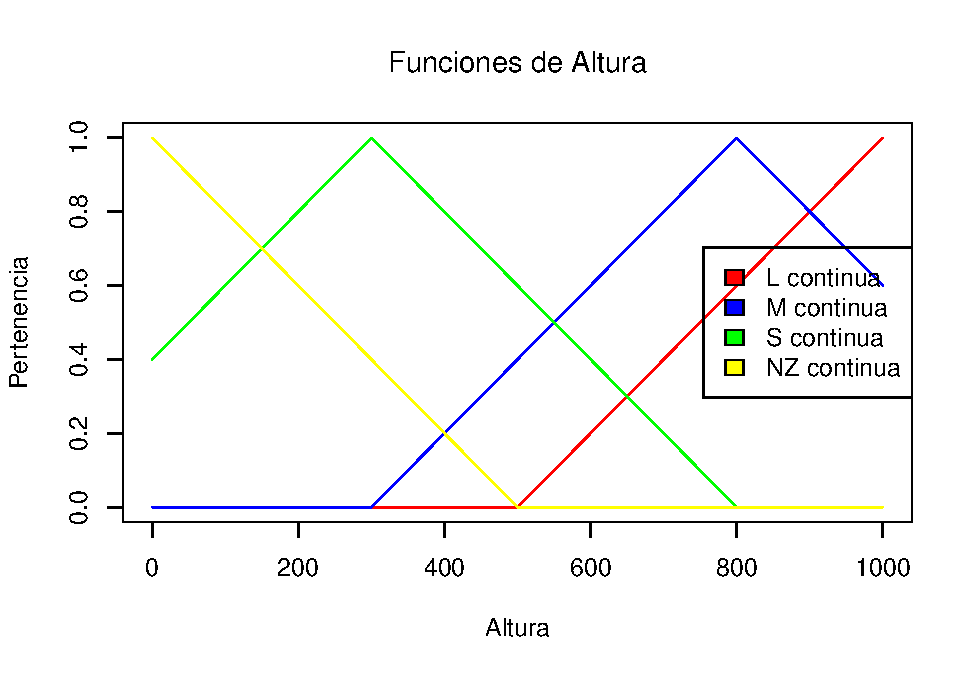
\includegraphics{tareaBloque3_files/figure-latex/unnamed-chunk-11-1.pdf}
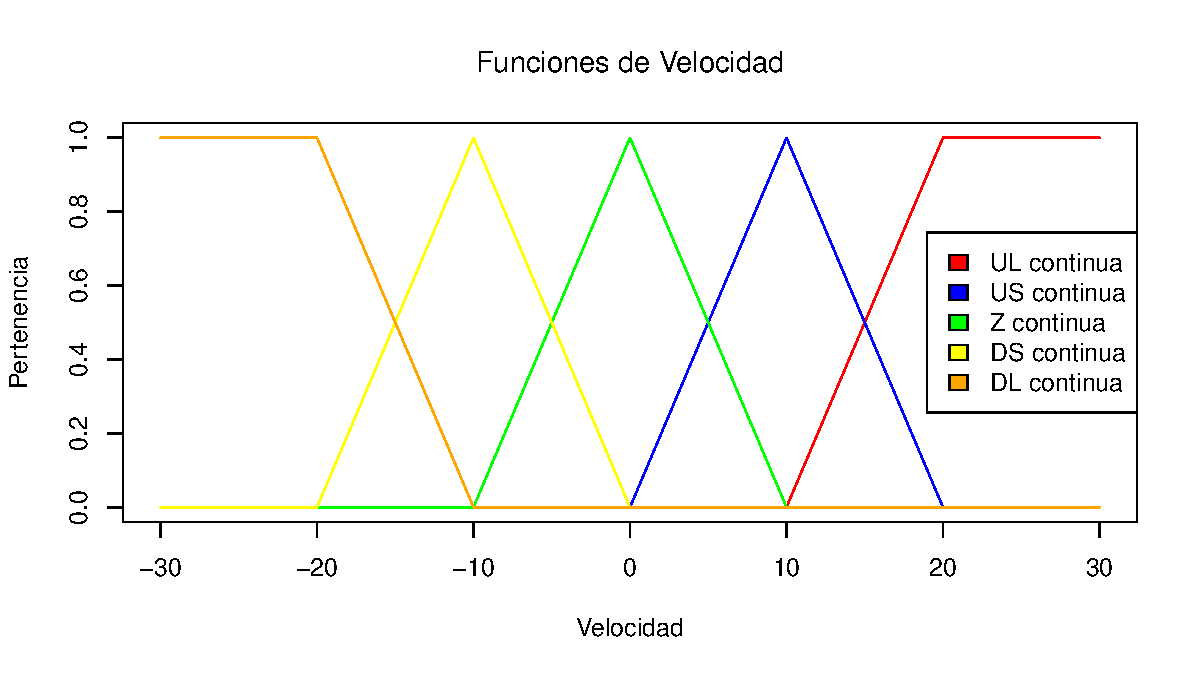
\includegraphics{tareaBloque3_files/figure-latex/unnamed-chunk-12-1.pdf}
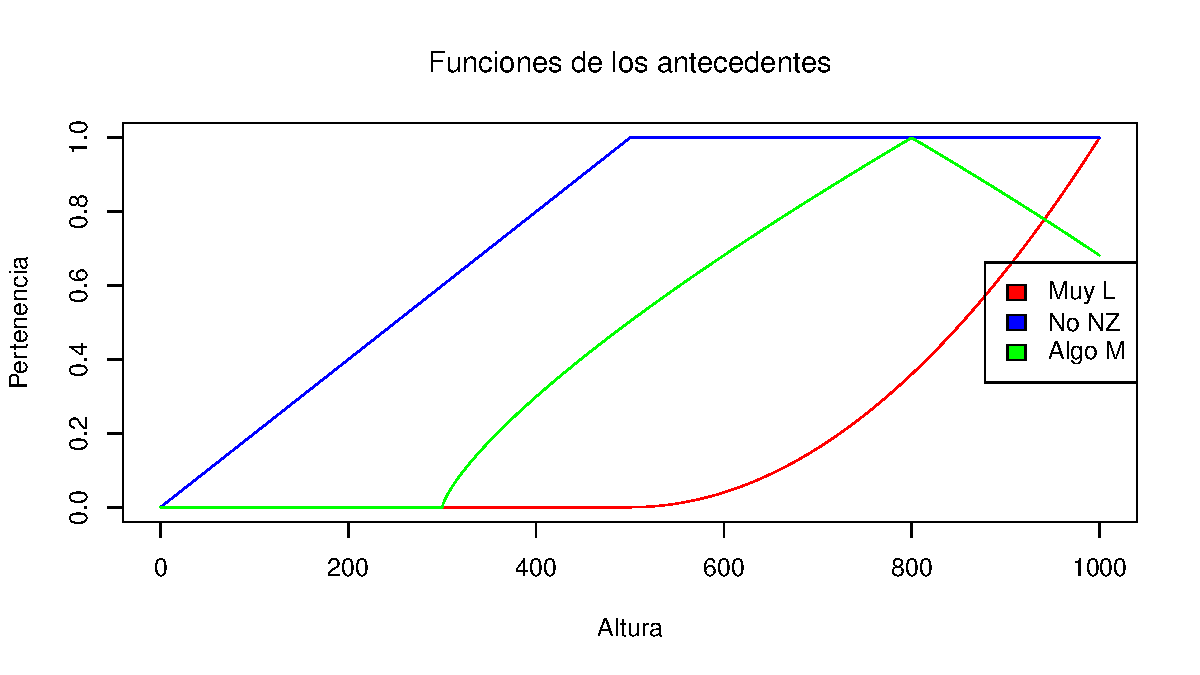
\includegraphics{tareaBloque3_files/figure-latex/unnamed-chunk-13-1.pdf}
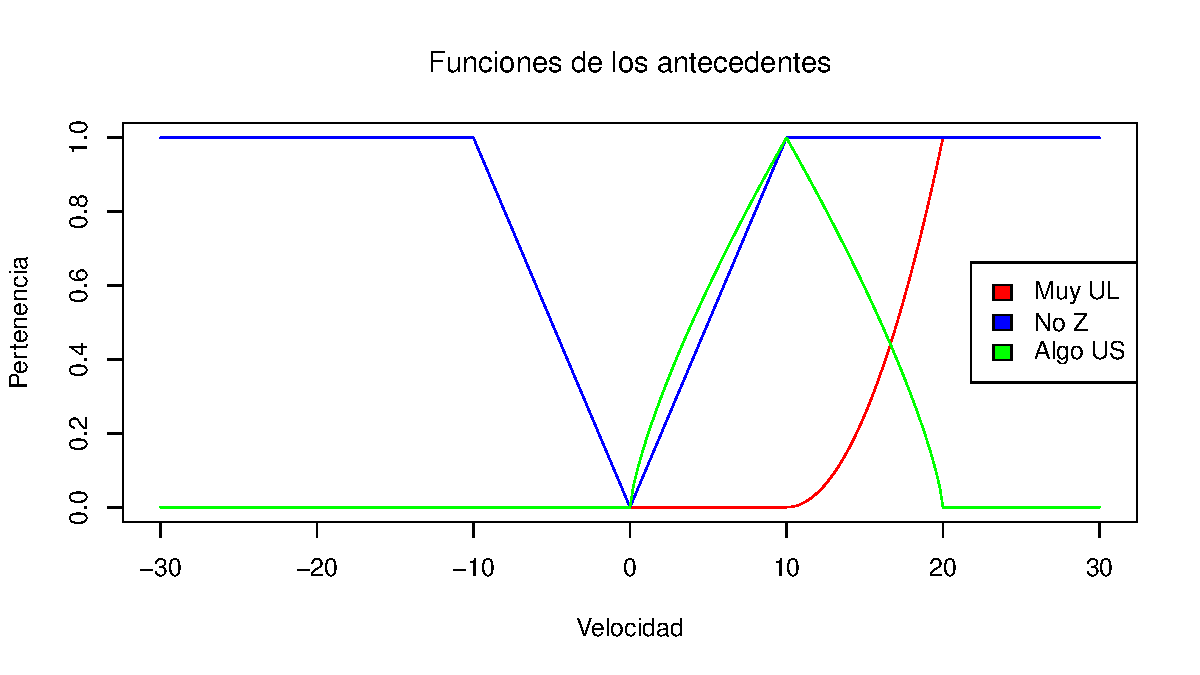
\includegraphics{tareaBloque3_files/figure-latex/unnamed-chunk-13-2.pdf}
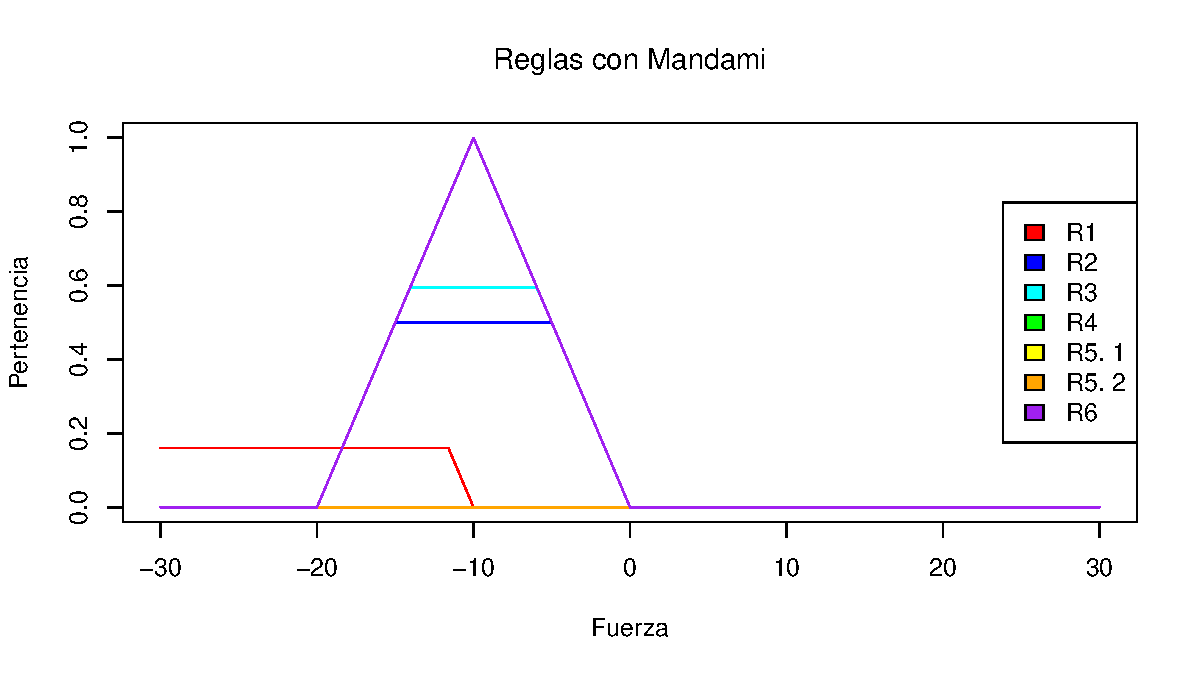
\includegraphics{tareaBloque3_files/figure-latex/unnamed-chunk-14-1.pdf}
Y para obtener el conjunto borroso final de la Fuerza, basta tomar el
máximo entre todas las reglas:
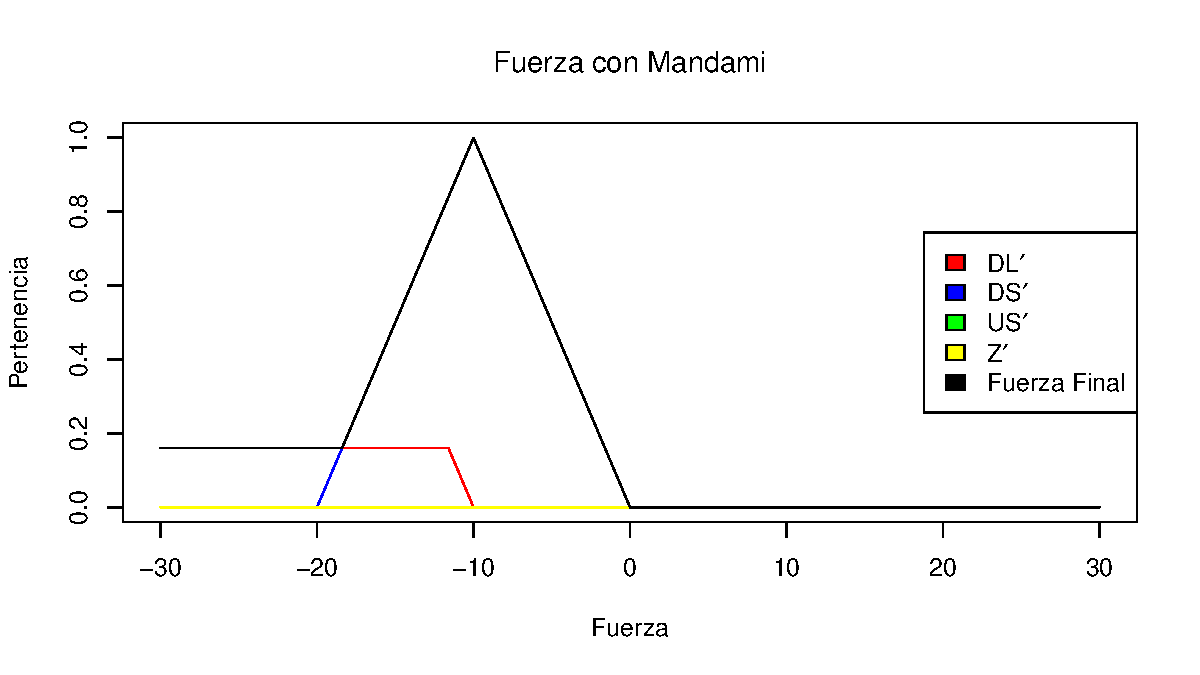
\includegraphics{tareaBloque3_files/figure-latex/unnamed-chunk-15-1.pdf}
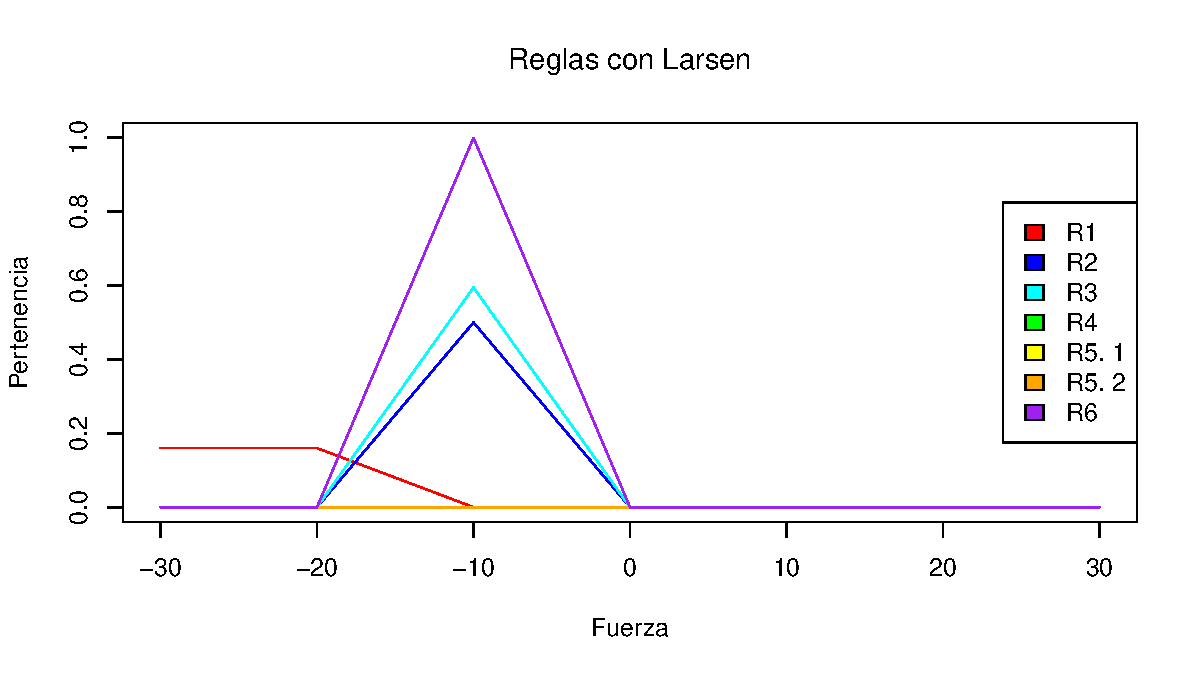
\includegraphics{tareaBloque3_files/figure-latex/unnamed-chunk-16-1.pdf}
Y para obtener el conjunto borroso final de la Fuerza, basta tomar el
máximo entre todas las reglas:
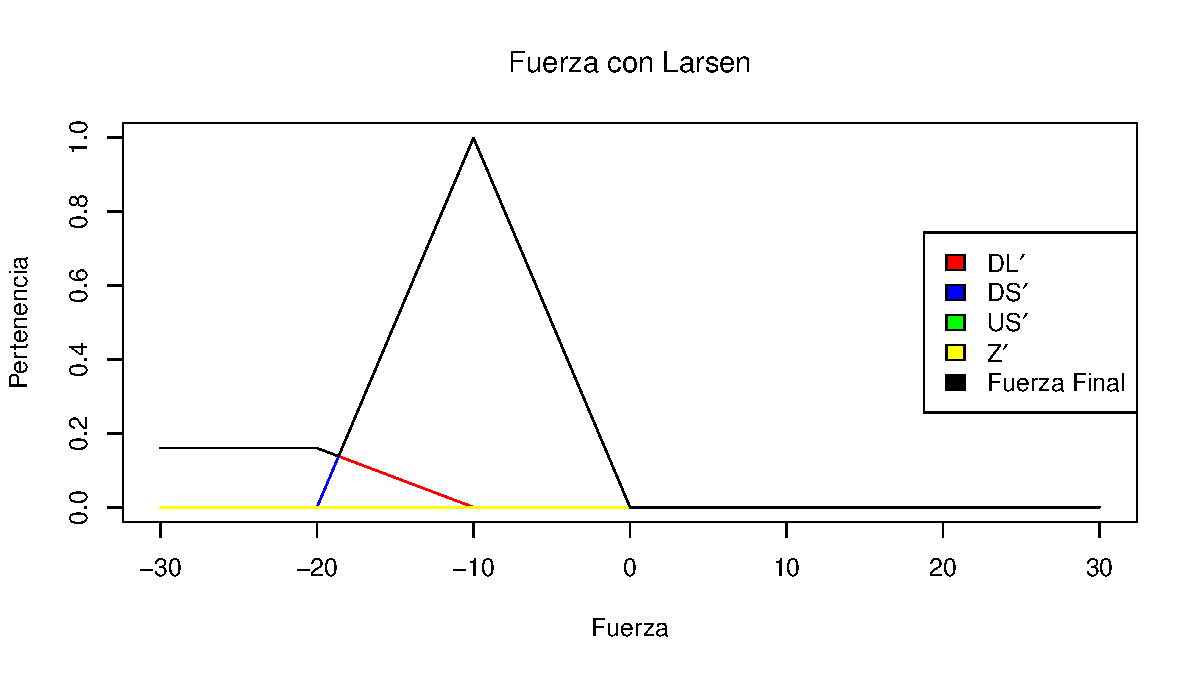
\includegraphics{tareaBloque3_files/figure-latex/unnamed-chunk-17-1.pdf}
Y solo queda calcular el centroide. En el caso continuo no es una suma
finita, como hicimos antes, sino que se hace mediante integrales:

\[y_{r}=\frac{\int_{V}y\mu_{B'}\left(y\right)dy}{\int_{V}\mu_{B'}\left(y\right)dy}\]

En el caso de Mandami:

\begin{Shaded}
\begin{Highlighting}[]
\NormalTok{xFM }\OtherTok{=} \ControlFlowTok{function}\NormalTok{(x) \{x}\SpecialCharTok{*}\FunctionTok{FM}\NormalTok{(x)\}}
\NormalTok{FMdefuzzy }\OtherTok{=} \FunctionTok{AUC}\NormalTok{(UV, }\FunctionTok{xFM}\NormalTok{(UV)) }\SpecialCharTok{/} \FunctionTok{AUC}\NormalTok{(UV,}\FunctionTok{FM}\NormalTok{(UV))}
\NormalTok{FMdefuzzy}
\end{Highlighting}
\end{Shaded}

\begin{verbatim}
## [1] -12.1498
\end{verbatim}

Y en el de Larsen:

\begin{Shaded}
\begin{Highlighting}[]
\NormalTok{xFL }\OtherTok{=} \ControlFlowTok{function}\NormalTok{(x) \{x}\SpecialCharTok{*}\FunctionTok{FL}\NormalTok{(x)\}}
\NormalTok{FLdefuzzy }\OtherTok{=} \FunctionTok{AUC}\NormalTok{(UV, }\FunctionTok{xFL}\NormalTok{(UV)) }\SpecialCharTok{/} \FunctionTok{AUC}\NormalTok{(UV,}\FunctionTok{FL}\NormalTok{(UV))}
\NormalTok{FLdefuzzy}
\end{Highlighting}
\end{Shaded}

\begin{verbatim}
## [1] -12.13958
\end{verbatim}

Obsérvese que en esta ocasión si que encontramos diferencias entre ambos
métodos, aunque todas las formas de hacerlo nos han dado resultados
bastante próximos.

\newpage

\hypertarget{problema-5}{%
\section{Problema 5}\label{problema-5}}

El problema de simulación del aterrizaje de los aviones descrito
anteriormente nos permitía obtener la fuerza que hay que aplicarle al
avión dada una altitud y velocidad determinadas. Una vez determinada la
fuerza, la nueva velocidad y altitud se calculan mediante las siguientes
expresiones: \[v_{i+1}=v_{i}+f_{i}\] \[h_{i+1}=h_{i}+v_{i}\] donde
\(v_{i+1}\) y \(h_{i+1}\) son la nueva velocidad y altitud
respectivamente una vez apicada una fuerza \(f_{i}\) a un avión con una
altitud \(h_{i}\) y una velocidad de descenso \(v_{i}\), siendo
\(v_{0}\) y \(h_{0}\) los valores iniciales de velocidad y altitud. Se
pide:

\begin{enumerate}
\def\labelenumi{\arabic{enumi}.}
\item
  Partiendo del sistema definido en el apartado anterior, y para los
  mismos valores de entrada, resolver con JFuzzyLogic el problema
  anterior para los mismos valores de entrada, pero sustituyendo el
  conjunto de reglas por las siguientes reglas:

  \begin{table}[H]
  \centering
  \begin{tabular}{|l|llllll|}
  \hline
                                 & \multicolumn{6}{l|}{\textbf{Velocidad de descenso}}                                                                                                                                       \\ \hline
  \multirow{5}{*}{\textbf{Altitud}} & \multicolumn{1}{l|}{}            & \multicolumn{1}{l|}{\textbf{DL}} & \multicolumn{1}{l|}{\textbf{DS}} & \multicolumn{1}{l|}{\textbf{Z}} & \multicolumn{1}{l|}{\textbf{US}} & \textbf{UL} \\ \cline{2-7} 
                                 & \multicolumn{1}{l|}{\textbf{L}}  & \multicolumn{1}{l|}{Z}           & \multicolumn{1}{l|}{DS}          & \multicolumn{1}{l|}{DL}         & \multicolumn{1}{l|}{DL}          & DL          \\ \cline{2-7} 
                                 & \multicolumn{1}{l|}{\textbf{M}}  & \multicolumn{1}{l|}{US}          & \multicolumn{1}{l|}{Z}           & \multicolumn{1}{l|}{DS}         & \multicolumn{1}{l|}{DL}          & DL          \\ \cline{2-7} 
                                 & \multicolumn{1}{l|}{\textbf{S}}  & \multicolumn{1}{l|}{UL}          & \multicolumn{1}{l|}{US}          & \multicolumn{1}{l|}{Z}          & \multicolumn{1}{l|}{DS}          & DL          \\ \cline{2-7} 
                                 & \multicolumn{1}{l|}{\textbf{NZ}} & \multicolumn{1}{l|}{UL}          & \multicolumn{1}{l|}{UL}          & \multicolumn{1}{l|}{Z}          & \multicolumn{1}{l|}{DS}          & DS          \\ \hline
  \end{tabular}
  \end{table}

  Adjuntar las imágenes en las que se puedan apreciar cómo están
  definidas las diferentes variables borrosas y el resultado de la
  evaluación de las reglas.
\item
  Realizar una aplicación, utilizando JFuzzyLogic, que realice la
  simulación del aterrizaje del avión. Para ello nos basaremos en el SIB
  definido a aprtir de las reglas del apartado anterior y de las
  ecuaciones de estado indicadas al comienzo del problema. Considerar
  que los incrementos de tiempos son de un segundo.
\item
  El resultado de la simulación se puede presentar de la siguiente
  forma:

  \begin{enumerate}
  \def\labelenumii{\alph{enumii}.}
  \item
    A través del terminal de eclipse imprimiendo en cada línea la
    evolución de cada parámetro
  \item
    Mediante gráficas que muestren la evolución de los parámetros
  \item
    Mediante simulación animada del proceso de aterrizaje
  \end{enumerate}
\end{enumerate}

Para realizar este ejercicio, defino las variables de entrada y salida:

\begin{lstlisting}[language=Java, caption=Definición de variables de entrada y salida]
FUNCTION_BLOCK aterrizaje   

VAR_INPUT               
    altura : REAL;
    velocidad : REAL;
END_VAR

VAR_OUTPUT              
    fuerza : REAL;
END_VAR
\end{lstlisting}

Y los conjuntos borrosos:

\begin{lstlisting}[language=Java, caption=Definición de los conjuntos borrosos]
FUZZIFY altura          
    TERM L := (500, 0) (600, 0.2) (700, 0.4) (800, 0.6) (900, 0.8) (1000, 1) ; 
    TERM M := (300, 0) (400, 0.2) (500, 0.4) (600, 0.6) (700, 0.8) (800, 1) (900, 0.8) (1000, 0.6) ; 
    TERM S := (0, 0.4) (100, 0.6) (200, 0.8) (300, 1) (400, 0.8) (500, 0.6) (600, 0.4) (700, 0.2) ;
    TERM NZ := (0, 1) (100, 0.8) (200, 0.6) (300, 0.4) (400, 0.2) (500, 0) ;  
END_FUZZIFY

FUZZIFY velocidad           
    TERM UL := (10, 0) (15, 0.5) (20, 1) (25, 1) (30, 1) ;
    TERM US := (0, 0) (5, 0.5) (10, 1) (15, 0.5) (20, 0) ;
    TERM Z := (-10, 0) (-5, 0.5) (0, 1) (5, 0.5) (10, 0) ;
    TERM DS := (-20, 0) (-15, 0.5) (-10, 1) (-5, 0.5) (0, 0) ;
    TERM DL := (-30, 1) (-25, 1) (-20, 1) (-15, 0.5) (-10, 0) ;
END_FUZZIFY

DEFUZZIFY fuerza            
    TERM UL := (10, 0) (15, 0.5) (20, 1) (25, 1) (30, 1) ;
    TERM US := (0, 0) (5, 0.5) (10, 1) (15, 0.5) (20, 0) ;
    TERM Z := (-10, 0) (-5, 0.5) (0, 1) (5, 0.5) (10, 0) ;
    TERM DS := (-20, 0) (-15, 0.5) (-10, 1) (-5, 0.5) (0, 0) ;
    TERM DL := (-30, 1) (-25, 1) (-20, 1) (-15, 0.5) (-10, 0) ;
    METHOD : COG;       // Centro de Gravedad para defuzzificar
    DEFAULT := 0;       
END_DEFUZZIFY
\end{lstlisting}

Por último, las reglas:

\begin{lstlisting}[language=Java, caption=Definición de variables de reglas]
RULEBLOCK Enunciado
    AND : MIN;          
    ACT : MIN;          
    ACCU : MAX;         

    RULE 1 : IF altura IS L AND velocidad IS DL THEN fuerza IS Z;
    RULE 2 : IF altura IS L AND velocidad IS DS THEN fuerza IS DS; 
    RULE 3 : IF altura IS L AND velocidad IS Z THEN fuerza IS DL;
    RULE 4 : IF altura IS L AND velocidad IS US THEN fuerza IS DL;
    RULE 5 : IF altura IS L AND velocidad IS UL THEN fuerza IS DL;
    RULE 6 : IF altura IS M AND velocidad IS DL THEN fuerza IS US; 
    RULE 7 : IF altura IS M AND velocidad IS DS THEN fuerza IS Z; 
    RULE 8 : IF altura IS M AND velocidad IS Z THEN fuerza IS DL;
    RULE 9 : IF altura IS M AND velocidad IS US THEN fuerza IS DL;
    RULE 10 : IF altura IS M AND velocidad IS UL THEN fuerza IS DL;
    RULE 11 : IF altura IS S AND velocidad IS DL THEN fuerza IS UL; 
    RULE 12 : IF altura IS S AND velocidad IS DS THEN fuerza IS US; 
    RULE 13 : IF altura IS S AND velocidad IS Z THEN fuerza IS Z; 
    RULE 14 : IF altura IS S AND velocidad IS US THEN fuerza IS DS; 
    RULE 15 : IF altura IS S AND velocidad IS UL THEN fuerza IS DL; 
    RULE 16 : IF altura IS NZ AND velocidad IS DL THEN fuerza IS UL; 
    RULE 17 : IF altura IS NZ AND velocidad IS DS THEN fuerza IS UL; 
    RULE 18 : IF altura IS NZ AND velocidad IS Z THEN fuerza IS Z; 
    RULE 19 : IF altura IS NZ AND velocidad IS US THEN fuerza IS DS; 
    RULE 20 : IF altura IS NZ AND velocidad IS UL THEN fuerza IS DS; 
END_RULEBLOCK

END_FUNCTION_BLOCK
\end{lstlisting}

Para realizar la evaluación con los valores del ejercicio anterior,
simplemente hacemos:

\begin{lstlisting}[language=Java, caption=Definición de variables de reglas]
  FunctionBlock functionBlock = fis.getFunctionBlock(functionBlockName);
        // Show
        JFuzzyChart.get().chart(functionBlock);

        // Set inputs
        fis.setVariable("altura", 700);
        fis.setVariable("velocidad", 15);
        
        // Evaluate
        fis.evaluate();

        // Show output variable's chart
        Variable fuerza = functionBlock.getVariable("fuerza");
        JFuzzyChart.get().chart(fuerza, fuerza.getDefuzzifier(), true);
        
        // Print ruleSet
        //System.out.println(fis);
        
        // Print output
        System.out.println(fuerza);
\end{lstlisting}

Podemos ver las gráficas de los conjuntos difusos:

\begin{figure}
\centering
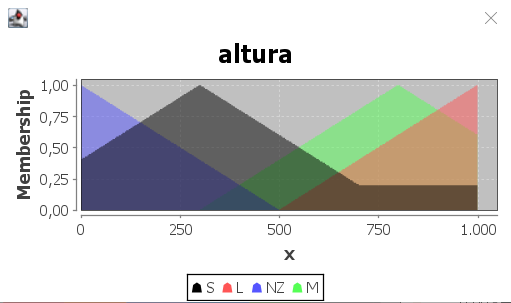
\includegraphics{pegado4.png}
\caption{Conjunto altura}
\end{figure}

\begin{figure}
\centering
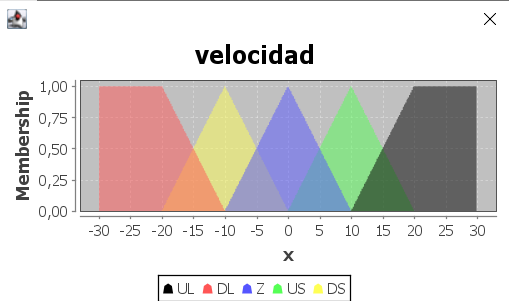
\includegraphics{pegado3.png}
\caption{Conjunto velocidad}
\end{figure}

\begin{figure}
\centering
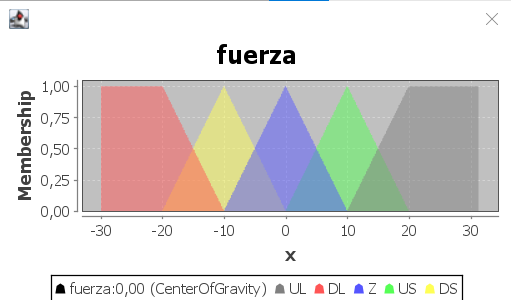
\includegraphics{pegado2.png}
\caption{Conjunto fuerza}
\end{figure}

Y al aplicar el centro de gravedad:

\begin{figure}
\centering
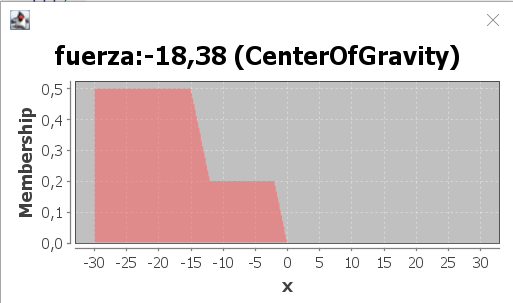
\includegraphics{pegado1.png}
\caption{Fuerza resultante}
\end{figure}

Para hacer la simulación del aterrizaje, basta hacer un bucle for en el
que vamos actualizando la altura y velocidad de cada iteración mediante
la fuerza calculada. Surge un problema, y es que con las reglas
proporcionadas el avión no aterriza, sino que se queda estable sobre los
320 metros. Intenté modificar las reglas, y lo mejor que conseguí fue
que se quedase estable en los 150 metros. Si conseguía hacer que llegase
a 0, seguía hacia abajo indefinidamente.

\begin{lstlisting}[language=Java, caption=Bucle para la simulación]
  static double h = 700;
    static double v = 15;
    static double f = 0.0;
    
    while(aterrizaje.size()<=200){ //Esperamos 200 segundos
        aterrizaje.add(h);
        
        fis.setVariable("altura", h);
        fis.setVariable("velocidad", v);
        
        fis.evaluate();
        
        fuerza = functionBlock.getVariable("fuerza");
        
        f = fuerza.getDefuzzifier().defuzzify();
        
        // Actualizamos los valores
        h=h+v;
        v=v+f;
        
    }
\end{lstlisting}

Esto hace la simulación, ahora debemos hacer las diferentes formas de
mostrar la información por pantalla.

La primera de ellas, mediante información textual, es muy sencilla.
Basta añadir, dentro del while, los comandos de impresión:

\begin{lstlisting}[language=Java, caption=Mostramos la información por pantalla]
  // imprimo la informacion
            System.out.println("Han pasado "+ aterrizaje.size() +" segundos");
            System.out.println("La altura es de " + h + " metros.");
            System.out.println("La velocidad vertical es de " + v + " m/s.");
            System.out.println("La fuerza a aplicar será de " + f + " libras.");
\end{lstlisting}

Para la segunda forma, mediante una gráfica, he creado una clase que
hereda de ApplicationFrame, a la que le pasas una lista de dobles, y te
la imprime por pantalla en forma de gráfica:

\begin{lstlisting}[language=Java, caption=Clase Plot]
public class Plot extends ApplicationFrame {

    private static final long serialVersionUID = 1L;

    public Plot(String title) {
        super(title);
    }
    
    public Plot (String title, LinkedList<Double> aterrizaje) {
        super(title);
        XYSeries series = new XYSeries("Aterrizaje");
        for(int t=0; t<aterrizaje.size(); t++) {
            series.add(t, aterrizaje.get(t));
        }
        XYSeriesCollection data = new XYSeriesCollection(series);
        JFreeChart chart = ChartFactory.createXYLineChart(
                "Aterrizaje",
                "Tiempo (en s)", 
                "Altura (en ft)", 
                data,
                PlotOrientation.VERTICAL,
                true,
                true,
                false
           );
        ChartPanel chartPanel = new ChartPanel(chart);
        chartPanel.setPreferredSize(new java.awt.Dimension(500, 270));
        setContentPane(chartPanel);
    }
}
\end{lstlisting}

Así, basta crear una lista de este tipo antes del bucle, e ir
llenándola. Al finalizar el bucle se la pasamos a Plot y le indicamos
que la imprima:

\begin{lstlisting}[language=Java, caption=Uso de la clase Plot para imprimir la gráfica del aterrizaje]
  LinkedList<Double> aterrizaje = new LinkedList<Double>();
    while(aterrizaje.size()<=200){ //Esperamos 200 segundos
        aterrizaje.add(h);
    
    ...
    //Calculamos los valores nuevos
    ...
        
        // Actualizamos los valores
        h=h+v;
        v=v+f;
        
    }
    
    Plot aterrizajePlot = new Plot("Aterrizaje", aterrizaje);
    aterrizajePlot.pack();
    RefineryUtilities.centerFrameOnScreen(aterrizajePlot);
    aterrizajePlot.setVisible(true);
\end{lstlisting}

El resultado obtenido es la siguiente gráfica:

\begin{figure}
\centering
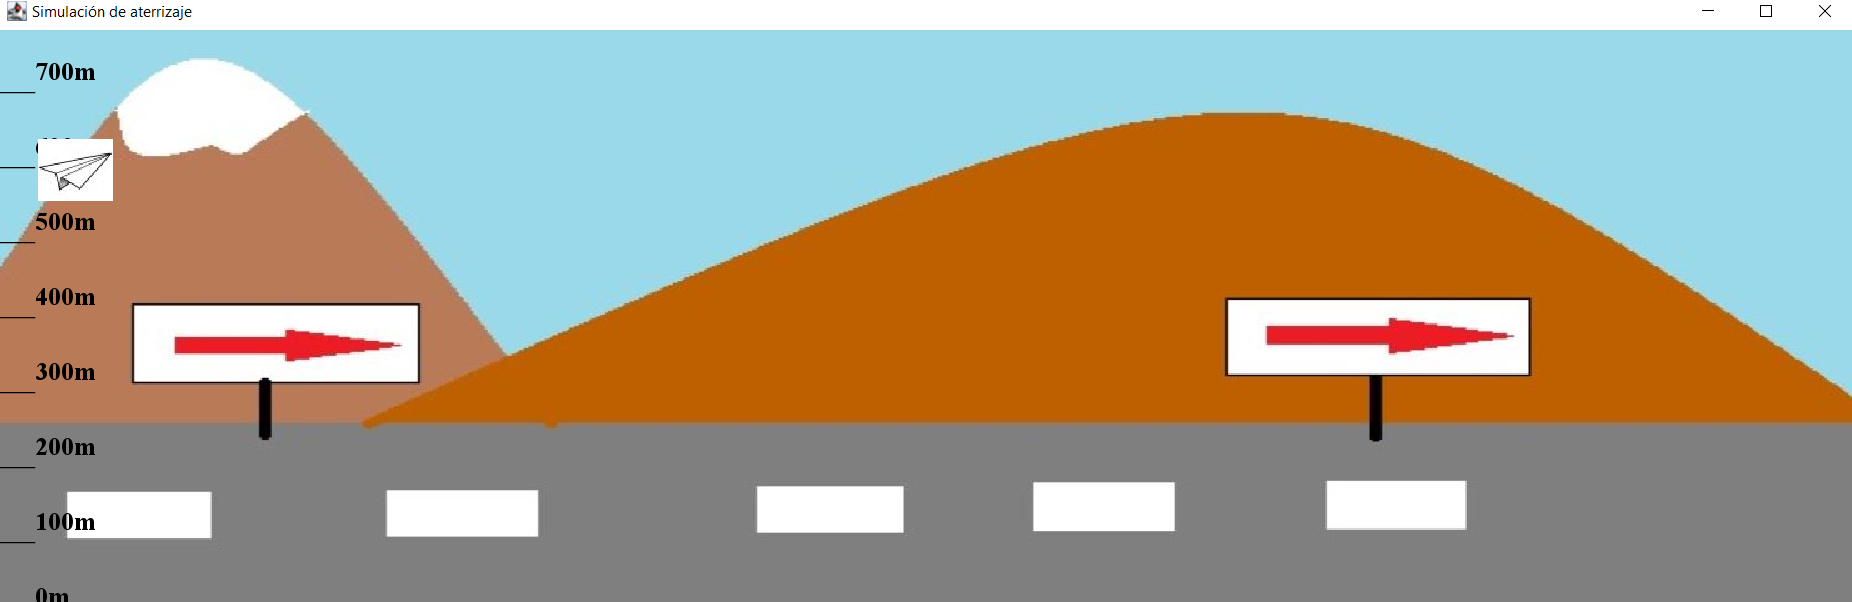
\includegraphics{pegado6.png}
\caption{Gráfica de la simulación}
\end{figure}

Por último, para la animación, creo un fondo sencillo (y un poco cutre,
hecho con paint, pero es gracioso) en el que se indican las diferentes
alturas. Una imagen de un avión va moviéndose, simplemente repintando el
fondo y la imagen:

\begin{lstlisting}[language=Java, caption=Dibujamos el fondo y la imagen]
  public void paint(Graphics g) {
        super.paint(g);
        g.setColor(Color.WHITE);
        g.fillRect(0,  0,  1500,  500);
        Graphics2D g2d = (Graphics2D) g;
        g2d.setRenderingHint(RenderingHints.KEY_ANTIALIASING, RenderingHints.VALUE_ANTIALIAS_ON);
        
        //Dibujamos el fondo
        g.drawImage(fondo, 0, 0, null);
        
        //Marcamos las alturas
        g.setColor(Color.BLACK);
        g2d.fillRect(0, 50, 30, 1);
        g2d.setFont(new Font("TimesRoman", Font.BOLD, 20));
        g2d.drawString("700m", 30, 40);
        g2d.fillRect(0, 110, 30, 1);
        g2d.drawString("600m", 30, 100);
        g2d.fillRect(0, 170, 30, 1);
        g2d.drawString("500m", 30, 160);
        g2d.fillRect(0, 230, 30, 1);
        g2d.drawString("400m", 30, 220);
        g2d.fillRect(0, 290, 30, 1);
        g2d.drawString("300m", 30, 280);
        g2d.fillRect(0, 350, 30, 1);
        g2d.drawString("200m", 30, 340);
        g2d.fillRect(0, 410, 30, 1);
        g2d.drawString("100m", 30, 400);
        g2d.fillRect(0, 470, 30, 1);
        g2d.drawString("0m", 30, 460);
        
        //Dibujamos la imagen
        g.drawImage(image, y, 500-(int)(h*5/7), null);
    }
\end{lstlisting}

Tengo también una función, \(movePlane\), que simplemente se encarga de
cambiar la posición horizontal del avión, la \(y\) de la función
anterior al dibujar \(image\).

Y dentro del bucle vamos redibujando:

\begin{lstlisting}[language=Java, caption=Dibujamos el fondo y la imagen]
  frame = new JFrame("Simulación de aterrizaje");
    Tarea3 t = new Tarea3();
    frame.add(t);
    frame.setSize(1500, 500);
    frame.setVisible(true);
    frame.setDefaultCloseOperation(JFrame.EXIT_ON_CLOSE);
    Thread.sleep(2000);
    
    while(aterrizaje.size()<=200){ //Esperamos 200 segundos
        ...
        //Calculamos los valores
        ...
        
        // hacemos el efecto de la animacion
        
        //movemos horizontalmente el avión
        t.movePlane();
        
        //Repintamos todo
        frame.getContentPane().setBackground(Color.YELLOW);
        t.repaint();
           
        //Para que no sea demasiado rápido
        t.revalidate();
        Thread.sleep(50);
        
        // Actualizamos los valores
        h=h+v;
        v=v+f;
        
    }
\end{lstlisting}

Un par de capturas de la animación:

\begin{figure}
\centering
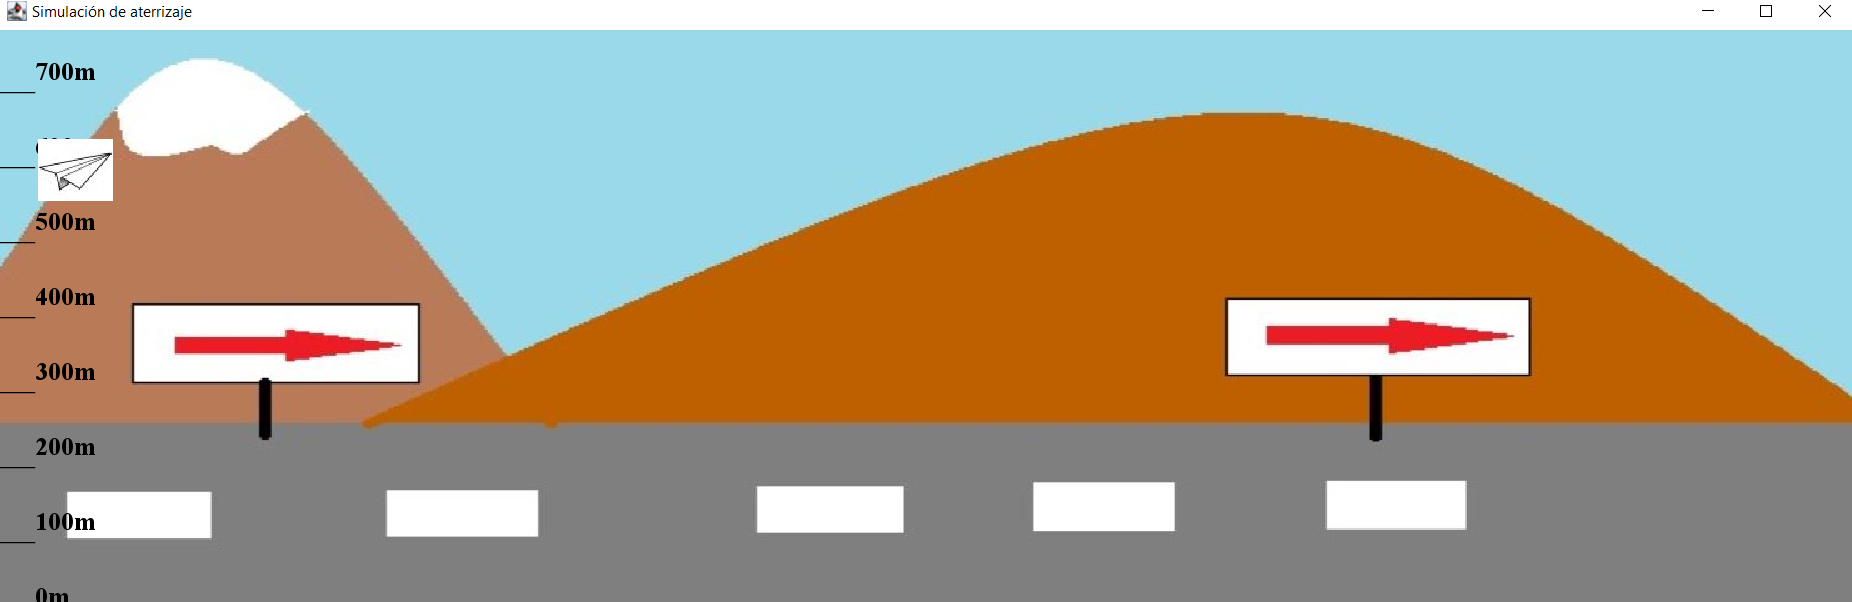
\includegraphics{pegado6.png}
\caption{Animación de aterrizaje}
\end{figure}

\begin{figure}
\centering
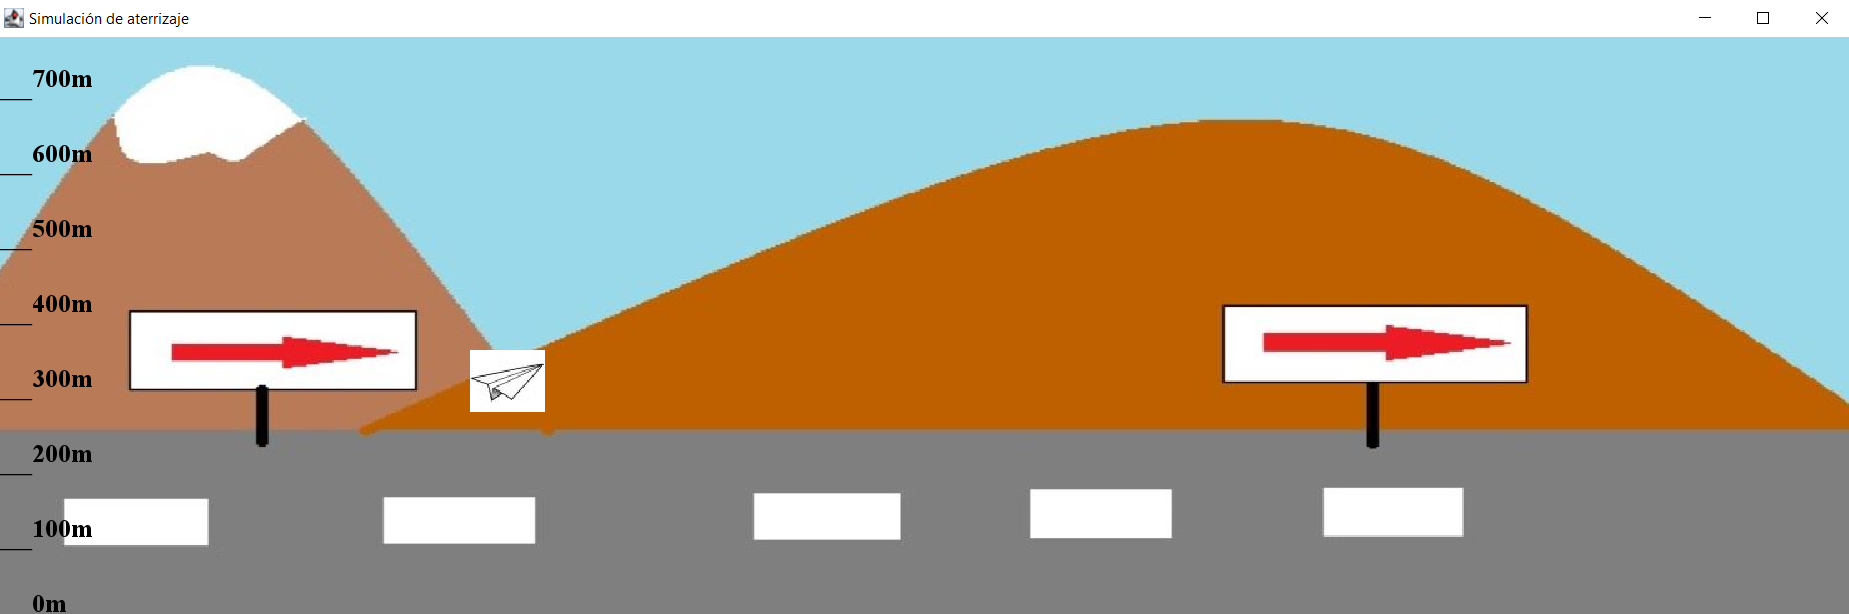
\includegraphics{pegado7.png}
\caption{Animación de aterrizaje}
\end{figure}

\newpage

\hypertarget{bibliografuxeda}{%
\section{Bibliografía}\label{bibliografuxeda}}

\hypertarget{refs}{}
\begin{CSLReferences}{0}{0}
\leavevmode\hypertarget{ref-PalmaConjuntosBorrosos}{}%
1. Palma JT. Conjuntos borrosos. 2013.

\leavevmode\hypertarget{ref-BotiaConjuntosBorrosos}{}%
2. Botia JA. Ejercicios ejemplo de conjuntos borrosos. 2021.

\leavevmode\hypertarget{ref-Stanford}{}%
3. Stanford. The law of excluded middle. An Introduction to Philosophy
{[}Internet{]}. Available from:
\url{https://web.stanford.edu/~bobonich/glances\%20ahead/IV.excluded.middle.html}

\leavevmode\hypertarget{ref-PalmaLogicaBorrosa}{}%
4. Palma JT. Logica e inferencia borrosos. 2017.

\leavevmode\hypertarget{ref-BotiaPalmaImplicaciones}{}%
5. Juan A. Botia JTP. Tipos de implicaciones y DOF. 2020.

\leavevmode\hypertarget{ref-PalmaInferencia}{}%
6. Palma JT. Sistemas de inferencia borrosa.

\leavevmode\hypertarget{ref-BotiaPalmaInferencia}{}%
7. Juan A. Botia JTP. Inferencia borrosa.

\end{CSLReferences}

\end{document}
